%% bare_jrnl.tex
%% V1.4b
%% 2015/08/26
%% by Michael Shell
%% see http://www.michaelshell.org/
%% for current contact information.
%%
%% This is a skeleton file demonstrating the use of IEEEtran.cls
%% (requires IEEEtran.cls version 1.8b or later) with an IEEE
%% journal paper.
%%
%% Support sites:
%% http://www.michaelshell.org/tex/ieeetran/
%% http://www.ctan.org/pkg/ieeetran
%% and
%% http://www.ieee.org/

%%*************************************************************************
%% Legal Notice:
%% This code is offered as-is without any warranty either expressed or
%% implied; without even the implied warranty of MERCHANTABILITY or
%% FITNESS FOR A PARTICULAR PURPOSE!
%% User assumes all risk.
%% In no event shall the IEEE or any contributor to this code be liable for
%% any damages or losses, including, but not limited to, incidental,
%% consequential, or any other damages, resulting from the use or misuse
%% of any information contained here.
%%
%% All comments are the opinions of their respective authors and are not
%% necessarily endorsed by the IEEE.
%%
%% This work is distributed under the LaTeX Project Public License (LPPL)
%% ( http://www.latex-project.org/ ) version 1.3, and may be freely used,
%% distributed and modified. A copy of the LPPL, version 1.3, is included
%% in the base LaTeX documentation of all distributions of LaTeX released
%% 2003/12/01 or later.
%% Retain all contribution notices and credits.
%% ** Modified files should be clearly indicated as such, including  **
%% ** renaming them and changing author support contact information. **
%%*************************************************************************


% *** Authors should verify (and, if needed, correct) their LaTeX system  ***
% *** with the testflow diagnostic prior to trusting their LaTeX platform ***
% *** with production work. The IEEE's font choices and paper sizes can   ***
% *** trigger bugs that do not appear when using other class files.       ***                          ***
% The testflow support page is at:
% http://www.michaelshell.org/tex/testflow/



\documentclass[journal]{IEEEtran}
%
% If IEEEtran.cls has not been installed into the LaTeX system files,
% manually specify the path to it like:
% \documentclass[journal]{../sty/IEEEtran}





% Some very useful LaTeX packages include:
% (uncomment the ones you want to load)


% *** MISC UTILITY PACKAGES ***
%
%\usepackage{ifpdf}
% Heiko Oberdiek's ifpdf.sty is very useful if you need conditional
% compilation based on whether the output is pdf or dvi.
% usage:
% \ifpdf
%   % pdf code
% \else
%   % dvi code
% \fi
% The latest version of ifpdf.sty can be obtained from:
% http://www.ctan.org/pkg/ifpdf
% Also, note that IEEEtran.cls V1.7 and later provides a builtin
% \ifCLASSINFOpdf conditional that works the same way.
% When switching from latex to pdflatex and vice-versa, the compiler may
% have to be run twice to clear warning/error messages.






% *** CITATION PACKAGES ***
%
% *** CITATION PACKAGES ***
%
\usepackage{amsmath}
\usepackage{amssymb}
\usepackage{bm}
\usepackage{cite}
\usepackage{graphicx}
\usepackage{multirow}
\usepackage{booktabs}
\usepackage{threeparttable}
%\usepackage{cite}
% cite.sty was written by Donald Arseneau
% V1.6 and later of IEEEtran pre-defines the format of the cite.sty package
% \cite{} output to follow that of the IEEE. Loading the cite package will
% result in citation numbers being automatically sorted and properly
% "compressed/ranged". e.g., [1], [9], [2], [7], [5], [6] without using
% cite.sty will become [1], [2], [5]--[7], [9] using cite.sty. cite.sty's
% \cite will automatically add leading space, if needed. Use cite.sty's
% noadjust option (cite.sty V3.8 and later) if you want to turn this off
% such as if a citation ever needs to be enclosed in parenthesis.
% cite.sty is already installed on most LaTeX systems. Be sure and use
% version 5.0 (2009-03-20) and later if using hyperref.sty.
% The latest version can be obtained at:
% http://www.ctan.org/pkg/cite
% The documentation is contained in the cite.sty file itself.






% *** GRAPHICS RELATED PACKAGES ***
%
\ifCLASSINFOpdf
  % \usepackage[pdftex]{graphicx}
  % declare the path(s) where your graphic files are
  % \graphicspath{{../pdf/}{../jpeg/}}
  % and their extensions so you won't have to specify these with
  % every instance of \includegraphics
  % \DeclareGraphicsExtensions{.pdf,.jpeg,.png}
\else
  % or other class option (dvipsone, dvipdf, if not using dvips). graphicx
  % will default to the driver specified in the system graphics.cfg if no
  % driver is specified.
  % \usepackage[dvips]{graphicx}
  % declare the path(s) where your graphic files are
  % \graphicspath{{../eps/}}
  % and their extensions so you won't have to specify these with
  % every instance of \includegraphics
  % \DeclareGraphicsExtensions{.eps}
\fi
% graphicx was written by David Carlisle and Sebastian Rahtz. It is
% required if you want graphics, photos, etc. graphicx.sty is already
% installed on most LaTeX systems. The latest version and documentation
% can be obtained at:
% http://www.ctan.org/pkg/graphicx
% Another good source of documentation is "Using Imported Graphics in
% LaTeX2e" by Keith Reckdahl which can be found at:
% http://www.ctan.org/pkg/epslatex
%
% latex, and pdflatex in dvi mode, support graphics in encapsulated
% postscript (.eps) format. pdflatex in pdf mode supports graphics
% in .pdf, .jpeg, .png and .mps (metapost) formats. Users should ensure
% that all non-photo figures use a vector format (.eps, .pdf, .mps) and
% not a bitmapped formats (.jpeg, .png). The IEEE frowns on bitmapped formats
% which can result in "jaggedy"/blurry rendering of lines and letters as
% well as large increases in file sizes.
%
% You can find documentation about the pdfTeX application at:
% http://www.tug.org/applications/pdftex





% *** MATH PACKAGES ***
%
%\usepackage{amsmath}
% A popular package from the American Mathematical Society that provides
% many useful and powerful commands for dealing with mathematics.
%
% Note that the amsmath package sets \interdisplaylinepenalty to 10000
% thus preventing page breaks from occurring within multiline equations. Use:
%\interdisplaylinepenalty=2500
% after loading amsmath to restore such page breaks as IEEEtran.cls normally
% does. amsmath.sty is already installed on most LaTeX systems. The latest
% version and documentation can be obtained at:
% http://www.ctan.org/pkg/amsmath





% *** SPECIALIZED LIST PACKAGES ***
%
%\usepackage{algorithmic}
% algorithmic.sty was written by Peter Williams and Rogerio Brito.
% This package provides an algorithmic environment fo describing algorithms.
% You can use the algorithmic environment in-text or within a figure
% environment to provide for a floating algorithm. Do NOT use the algorithm
% floating environment provided by algorithm.sty (by the same authors) or
% algorithm2e.sty (by Christophe Fiorio) as the IEEE does not use dedicated
% algorithm float types and packages that provide these will not provide
% correct IEEE style captions. The latest version and documentation of
% algorithmic.sty can be obtained at:
% http://www.ctan.org/pkg/algorithms
% Also of interest may be the (relatively newer and more customizable)
% algorithmicx.sty package by Szasz Janos:
% http://www.ctan.org/pkg/algorithmicx




% *** ALIGNMENT PACKAGES ***
%
%\usepackage{array}
% Frank Mittelbach's and David Carlisle's array.sty patches and improves
% the standard LaTeX2e array and tabular environments to provide better
% appearance and additional user controls. As the default LaTeX2e table
% generation code is lacking to the point of almost being broken with
% respect to the quality of the end results, all users are strongly
% advised to use an enhanced (at the very least that provided by array.sty)
% set of table tools. array.sty is already installed on most systems. The
% latest version and documentation can be obtained at:
% http://www.ctan.org/pkg/array


% IEEEtran contains the IEEEeqnarray family of commands that can be used to
% generate multiline equations as well as matrices, tables, etc., of high
% quality.




% *** SUBFIGURE PACKAGES ***
%\ifCLASSOPTIONcompsoc
%  \usepackage[caption=false,font=normalsize,labelfont=sf,textfont=sf]{subfig}
%\else
%  \usepackage[caption=false,font=footnotesize]{subfig}
%\fi
% subfig.sty, written by Steven Douglas Cochran, is the modern replacement
% for subfigure.sty, the latter of which is no longer maintained and is
% incompatible with some LaTeX packages including fixltx2e. However,
% subfig.sty requires and automatically loads Axel Sommerfeldt's caption.sty
% which will override IEEEtran.cls' handling of captions and this will result
% in non-IEEE style figure/table captions. To prevent this problem, be sure
% and invoke subfig.sty's "caption=false" package option (available since
% subfig.sty version 1.3, 2005/06/28) as this is will preserve IEEEtran.cls
% handling of captions.
% Note that the Computer Society format requires a larger sans serif font
% than the serif footnote size font used in traditional IEEE formatting
% and thus the need to invoke different subfig.sty package options depending
% on whether compsoc mode has been enabled.
%
% The latest version and documentation of subfig.sty can be obtained at:
% http://www.ctan.org/pkg/subfig




% *** FLOAT PACKAGES ***
%
%\usepackage{fixltx2e}
% fixltx2e, the successor to the earlier fix2col.sty, was written by
% Frank Mittelbach and David Carlisle. This package corrects a few problems
% in the LaTeX2e kernel, the most notable of which is that in current
% LaTeX2e releases, the ordering of single and double column floats is not
% guaranteed to be preserved. Thus, an unpatched LaTeX2e can allow a
% single column figure to be placed prior to an earlier double column
% figure.
% Be aware that LaTeX2e kernels dated 2015 and later have fixltx2e.sty's
% corrections already built into the system in which case a warning will
% be issued if an attempt is made to load fixltx2e.sty as it is no longer
% needed.
% The latest version and documentation can be found at:
% http://www.ctan.org/pkg/fixltx2e


%\usepackage{stfloats}
% stfloats.sty was written by Sigitas Tolusis. This package gives LaTeX2e
% the ability to do double column floats at the bottom of the page as well
% as the top. (e.g., "\begin{figure*}[!b]" is not normally possible in
% LaTeX2e). It also provides a command:
%\fnbelowfloat
% to enable the placement of footnotes below bottom floats (the standard
% LaTeX2e kernel puts them above bottom floats). This is an invasive package
% which rewrites many portions of the LaTeX2e float routines. It may not work
% with other packages that modify the LaTeX2e float routines. The latest
% version and documentation can be obtained at:
% http://www.ctan.org/pkg/stfloats
% Do not use the stfloats baselinefloat ability as the IEEE does not allow
% \baselineskip to stretch. Authors submitting work to the IEEE should note
% that the IEEE rarely uses double column equations and that authors should try
% to avoid such use. Do not be tempted to use the cuted.sty or midfloat.sty
% packages (also by Sigitas Tolusis) as the IEEE does not format its papers in
% such ways.
% Do not attempt to use stfloats with fixltx2e as they are incompatible.
% Instead, use Morten Hogholm'a dblfloatfix which combines the features
% of both fixltx2e and stfloats:
%
% \usepackage{dblfloatfix}
% The latest version can be found at:
% http://www.ctan.org/pkg/dblfloatfix




%\ifCLASSOPTIONcaptionsoff
%  \usepackage[nomarkers]{endfloat}
% \let\MYoriglatexcaption\caption
% \renewcommand{\caption}[2][\relax]{\MYoriglatexcaption[#2]{#2}}
%\fi
% endfloat.sty was written by James Darrell McCauley, Jeff Goldberg and
% Axel Sommerfeldt. This package may be useful when used in conjunction with
% IEEEtran.cls'  captionsoff option. Some IEEE journals/societies require that
% submissions have lists of figures/tables at the end of the paper and that
% figures/tables without any captions are placed on a page by themselves at
% the end of the document. If needed, the draftcls IEEEtran class option or
% \CLASSINPUTbaselinestretch interface can be used to increase the line
% spacing as well. Be sure and use the nomarkers option of endfloat to
% prevent endfloat from "marking" where the figures would have been placed
% in the text. The two hack lines of code above are a slight modification of
% that suggested by in the endfloat docs (section 8.4.1) to ensure that
% the full captions always appear in the list of figures/tables - even if
% the user used the short optional argument of \caption[]{}.
% IEEE papers do not typically make use of \caption[]'s optional argument,
% so this should not be an issue. A similar trick can be used to disable
% captions of packages such as subfig.sty that lack options to turn off
% the subcaptions:
% For subfig.sty:
% \let\MYorigsubfloat\subfloat
% \renewcommand{\subfloat}[2][\relax]{\MYorigsubfloat[]{#2}}
% However, the above trick will not work if both optional arguments of
% the \subfloat command are used. Furthermore, there needs to be a
% description of each subfigure *somewhere* and endfloat does not add
% subfigure captions to its list of figures. Thus, the best approach is to
% avoid the use of subfigure captions (many IEEE journals avoid them anyway)
% and instead reference/explain all the subfigures within the main caption.
% The latest version of endfloat.sty and its documentation can obtained at:
% http://www.ctan.org/pkg/endfloat
%
% The IEEEtran \ifCLASSOPTIONcaptionsoff conditional can also be used
% later in the document, say, to conditionally put the References on a
% page by themselves.




% *** PDF, URL AND HYPERLINK PACKAGES ***
%
%\usepackage{url}
% url.sty was written by Donald Arseneau. It provides better support for
% handling and breaking URLs. url.sty is already installed on most LaTeX
% systems. The latest version and documentation can be obtained at:
% http://www.ctan.org/pkg/url
% Basically, \url{my_url_here}.

\newcommand{\argmax}{\mathop{\rm arg\ max}\limits}


% *** Do not adjust lengths that control margins, column widths, etc. ***
% *** Do not use packages that alter fonts (such as pslatex).         ***
% There should be no need to do such things with IEEEtran.cls V1.6 and later.
% (Unless specifically asked to do so by the journal or conference you plan
% to submit to, of course. )


% correct bad hyphenation here
\hyphenation{op-tical net-works semi-conduc-tor}


\begin{document}
%
% paper title
% Titles are generally capitalized except for words such as a, an, and, as,
% at, but, by, for, in, nor, of, on, or, the, to and up, which are usually
% not capitalized unless they are the first or last word of the title.
% Linebreaks \\ can be used within to get better formatting as desired.
% Do not put math or special symbols in the title.
\title{Non-Gaussianity Detection of EEG Signals Based on a Multivariate Scale Mixture Model for Diagnosis of Epileptic Seizures}
%
%
% author names and IEEE memberships
% note positions of commas and nonbreaking spaces ( ~ ) LaTeX will not break
% a structure at a ~ so this keeps an author's name from being broken across
% two lines.
% use \thanks{} to gain access to the first footnote area
% a separate \thanks must be used for each paragraph as LaTeX2e's \thanks
% was not built to handle multiple paragraphs
%

\author{Akira~Furui${}^{*}$,~\IEEEmembership{Member,~IEEE,}
        Ryota~Onishi,
        Akihito~Takeuchi,
        Tomoyuki~Akiyama${}^{*}$,
        and~Toshio~Tsuji${}^{*}$,~\IEEEmembership{Member,~IEEE}% <-this % stops a space
\thanks{${}^{*}$A.~Furui, R.~Onishi, and ${}^{*}$T.~Tsuji are with the Graduate School of Engineering, Hiroshima University, Higashi-hiroshima, 739-8527 Japan (e-mail: akirafurui@hiroshima-u.ac.jp; tsuji@bsys.hiroshima-u.ac.jp).}% <-this % stops a space
\thanks{A.~Takeuchi is with the Department of Neonatology, Okayama Medical Center, National Hospital Organization.}
\thanks{${}^{*}$T.~Akiyama is with the Department of Child Neurology, Okayama University Hospital (e-mail: takiyama@okayama-u.ac.jp).}% <-this % stops a space
\thanks{Manuscript received April 19, 2005; revised August 26, 2015.}}
% note the % following the last \IEEEmembership and also \thanks -
% these prevent an unwanted space from occurring between the last author name
% and the end of the author line. i.e., if you had this:
%
% \author{....lastname \thanks{...} \thanks{...} }
%                     ^------------^------------^----Do not want these spaces!
%
% a space would be appended to the last name and could cause every name on that
% line to be shifted left slightly. This is one of those "LaTeX things". For
% instance, "\textbf{A} \textbf{B}" will typeset as "A B" not "AB". To get
% "AB" then you have to do: "\textbf{A}\textbf{B}"
% \thanks is no different in this regard, so shield the last } of each \thanks
% that ends a line with a % and do not let a space in before the next \thanks.
% Spaces after \IEEEmembership other than the last one are OK (and needed) as
% you are supposed to have spaces between the names. For what it is worth,
% this is a minor point as most people would not even notice if the said evil
% space somehow managed to creep in.



% The paper headers
\markboth{Journal of \LaTeX\ Class Files,~Vol.~14, No.~8, August~2015}%
{Shell \MakeLowercase{\textit{et al.}}: Bare Demo of IEEEtran.cls for IEEE Journals}
% The only time the second header will appear is for the odd numbered pages
% after the title page when using the twoside option.
%
% *** Note that you probably will NOT want to include the author's ***
% *** name in the headers of peer review papers.                   ***
% You can use \ifCLASSOPTIONpeerreview for conditional compilation here if
% you desire.




% If you want to put a publisher's ID mark on the page you can do it like
% this:
%\IEEEpubid{0000--0000/00\$00.00~\copyright~2015 IEEE}
% Remember, if you use this you must call \IEEEpubidadjcol in the second
% column for its text to clear the IEEEpubid mark.



% use for special paper notices
%\IEEEspecialpapernotice{(Invited Paper)}




% make the title area
\maketitle

% As a general rule, do not put math, special symbols or citations
% in the abstract or keywords.
\begin{abstract}
% Structured Abstract must be fewer than 250 words 
\textit{Objective:}
The detection of epileptic seizures from scalp electroencephalogram (EEG) signals can facilitate early diagnosis and treatment.
Previous studies suggested that the Gaussianity of EEG distributions changes depending on the presence or absence of seizures; however, there is no general EEG signal model that can explain such changes in distributions within a unified scheme.
\textit{Methods:}
This paper describes the formulation of a stochastic EEG model based on a multivariate scale mixture distribution; the model can represent changes in non-Gaussianity caused by stochastic fluctuations in EEG.
In addition, we propose a novel EEG analysis method by combining the model with a filter bank and introduce an index representing the non-Gaussianity latent in each EEG frequency band.
\textit{Results:}
We applied the proposed method to multichannel EEG data from twenty patients with focal epilepsy.
The results showed significant increases the proposed index during epileptic seizures, particularly in the high-frequency band.
The index calculated in the high-frequency band allowed highly accurate classification of seizure segments and non-seizure segments (area under the curve (AUC) = 0.881) using only a simple threshold, and significantly outperformed the conventional amplitude-based index (\textit{p} $<$ 0.001).
\textit{Conclusion:}
This study proposed a multivariate scale mixture distribution-based stochastic EEG model capable of representing non-Gaussianity associated with epileptic seizures.
In the high-frequency band, the proposed index shows the possibility of classification of epileptic seizures.
\textit{Significance:}
The proposed model can be used in various fields of EEG, and helps to characterize stochastic fluctuations of multichannel EEG signals.
% 243/250 words
\end{abstract}

% Note that keywords are not normally used for peerreview papers.
\begin{IEEEkeywords}
Electroencephalogram (EEG), stochastic model, stochastic fluctuation, multivariate scale mixture model, epileptic seizure, non-Gaussianity.
\end{IEEEkeywords}






% For peer review papers, you can put extra information on the cover
% page as needed:
% \ifCLASSOPTIONpeerreview
% \begin{center} \bfseries EDICS Category: 3-BBND \end{center}
% \fi
%
% For peerreview papers, this IEEEtran command inserts a page break and
% creates the second title. It will be ignored for other modes.
\IEEEpeerreviewmaketitle



\section{Introduction}
% The very first letter is a 2 line initial drop letter followed
% by the rest of the first word in caps.
%
% form to use if the first word consists of a single letter:
% \IEEEPARstart{A}{demo} file is ....
%
% form to use if you need the single drop letter followed by
% normal text (unknown if ever used by the IEEE):
% \IEEEPARstart{A}{}demo file is ....
%
% Some journals put the first two words in caps:
% \IEEEPARstart{T}{his demo} file is ....
%
% Here we have the typical use of a "T" for an initial drop letter
% and "HIS" in caps to complete the first word.
\IEEEPARstart{E}{pilepsy} is a chronic neurological disorder that is characterized by recurrent and unprovoked epileptic seizures caused by abnormal electric activities of brain neurons. It is reported that there are approximately 50 million epilepsy patients worldwide~\cite{WHO}.
Electroencephalogram (EEG) can record neuronal electric activities and is routinely utilized for the diagnosis of epilepsy. Especially prolonged EEG recording is a powerful tool to confirm an epileptic seizure when a patient is manifesting signs and/or symptoms that are difficult judge from clinical observation, or even when there are no visible symptoms.
It is important to recognize seizures early because prolonged seizures can lead to increased brain damage.
However, correct interpretation of EEG requires extensive training and EEG specialists may not be readily available in emergency settings. If there is a tool to aid non-expert clinicians to interpret EEG, early recognition and treatment of seizures can eventually improve neurological outcome.

Numerous studies have attempted to detect epileptic seizures quantitatively using EEGs, which are bioelectric signals that can be recorded from the scalp~\cite{Deburchgraeve2008,Subasi2005,kellaway1979precise,Panzica1999,fusco1993ictal,Acir2005,Greene2008}.
For example, Deburachgrave \textit{et al.} detected epileptic seizures based on EEG analysis that focused on the periodicity of high amplitude slow wave activity and sharp changes in amplitude during seizures~\cite{Deburchgraeve2008}.
Subasi \textit{et al.} also performed a frequency analysis using wavelet transformation to identify epileptic seizures~\cite{Subasi2005}.
However, in the above methods, it may be difficult to detect epileptic seizures by evaluating only the magnitude of the amplitude or the changes in frequency, because EEGs recorded during epileptic seizures will differ significantly owing to patient age and the type of epilepsy.
In addition, although these methods generally calculate the features and use appropriate discriminators for classification,
there are problems such as computational complexity and parameter adjustment.
Therefore, in this study, we consider the feature extraction and discriminator problems separately, and focus on the improvement of indicators as the first step to evaluate the discrimination performance by more simple methods such as thresholds.

Meanwhile, the probability distribution shapes of EEGs have been studied as a feature independent of amplitude~\cite{Saunders1963,Gonen2012,Campbell1967,Weiss1973,Nurujjaman2009,Charles1999}.
Previous studies typically assumed that EEG signals followed a steady Gaussian distribution~\cite{Saunders1963,Gonen2012}; however, after Campbell \textit{et al.} statistically indicated that EEG signals had non-Gaussian properties~\cite{Campbell1967}, various studies examined the probability distribution shapes of EEG signals, focusing on their Gaussianity~\cite{Gonen2012,Weiss1973,Nurujjaman2009,Charles1999}.
Although few previous studies investigated  the relationship between epileptic seizures and the Gaussianity of EEG signals, some studies reported that EEG signals during epileptic seizures follow a non-Gaussian distribution~\cite{Nurujjaman2009,Charles1999}.
However, these studies are only experimental reports, and currently there is no theoretical framework for quantitatively addressing the non-Gaussianity of EEG signals as a feature.

In this study, we assume that non-Gaussianity in EEG signals is caused by stochastic fluctuations in amplitude, and propose a multivariate scale mixture model that can estimate these fluctuations from recorded EEG signals.
In the proposed model, a scalp EEG signal recorded at a certain time using multichannel electrodes follows a multivariate Gaussian distribution, and its variance-covariance matrix is considered as a random variable that follows an inverse Wishart distribution.
Thereby, it allows evaluation of the stochastic fluctuation of the variance-covariance matrix corresponding to the EEG amplitude.
In addition, by combining this model with a filter bank, we develop an analysis method that can extract time-series stochastic fluctuations in each EEG frequency band as the feature.
In the simulation experiment, parameter estimation based on the proposed method is conducted on artificial data, and the error between true values and estimated values observed when conditions are changed is discussed.
In the analysis experiment, the proposed method is used to analyze EEG signals recorded during focal seizures.
We also verify the goodness-of-fit of the proposed model and investigate the correspondence between (1) estimated stochastic fluctuations of EEG signals and (2) diagnoses by an epileptologist.

The reminder of this paper is organized as follows: Section II outlines the structure of the multivariate scale mixture model, the parameter estimation method, and the EEG analysis method considering frequency characteristics. Section III details the simulation experiments and EEG analysis experiments.
Section IV presents the results of these experiments, and Section V provides related discussions. Finally, Section VI discusses the conclusions of this study.
% You must have at least 2 lines in the paragraph with the drop letter
% (should never be an issue)

\section{Methods}

\subsection{Multivariate Scale Mixture Model of Scalp EEG Signals}
Fig. \ref{fig:model} shows the stochastic relationship between the recorded EEG signal $\mathbf{x} \in \mathbb{R}^{D}$ ($D$ is the number of electrodes) and its variance-covariance matrix $\mathbf{\Sigma} \in \mathbb{R}^{D \times D}$ as a graphical model.
In the proposed model, $\mathbf{x}$ is handled as a random variable that follows a multivariate Gaussian distribution with a mean of zero and a variance-covariance matrix of $\mathbf{\Sigma}$.
The variance-covariance matrix $\mathbf{\Sigma}$ is also a random variable for which the distribution is determined by the degrees of freedom parameter $\nu \in \mathbb{R}^+$ and the scale matrix parameter $\mathbf{\Psi} \in \mathbb{R}^{D \times D}$.
Therefore, the variance-covariance matrix $\mathbf{\Sigma}$ is interpreted as a latent variable in the model.

%%%%%%%%%%%%%%%%%%%%%%%%%%%%%%%%
\begin{figure}[!t]
\centering
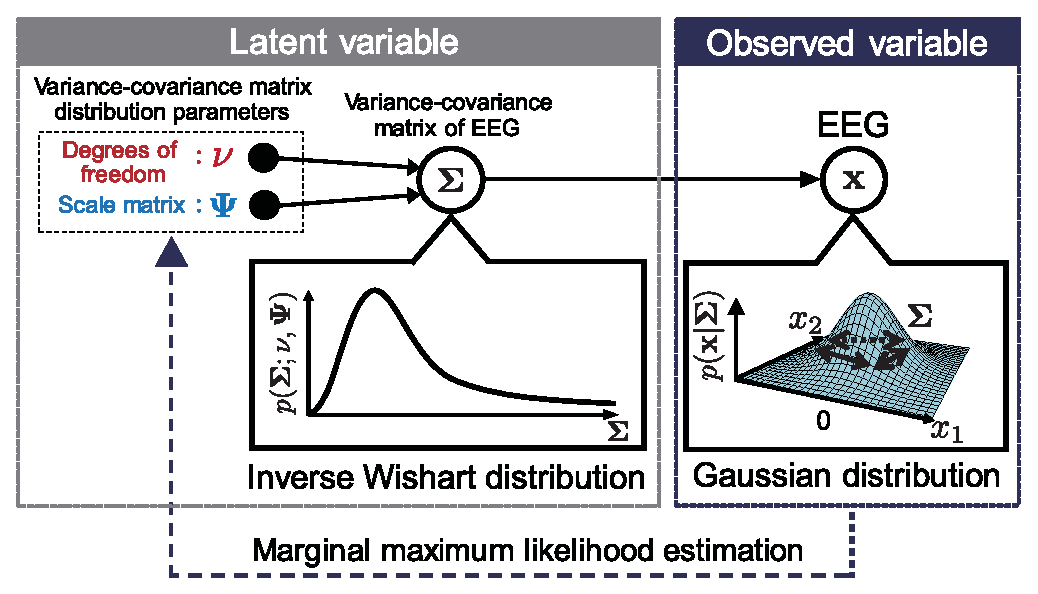
\includegraphics[width=1.0\hsize]{figure/fig1_ver2.eps}
%\end{center}
\caption{Graphical representation of the proposed multivariate scale mixture model, which describes the stochastic relationship between EEG signals and its variance-covariance matrix.
The white nodes are random variables and the black nodes are parameters to be estimated.
In the model, an EEG signal $\mathbf{x} \in \mathbb{R}^{D}$ is handled as a random variable that follows a multivariate Gaussian distribution with a mean vector of $\mathbf{0}$ and a variance-covariance matrix $\mathbf{\Sigma} \in \mathbb{R}^{D \times D}$ which is also a random variable following the inverse Wishart distribution determined by the degrees of freedom $\nu \in \mathbb{R}^+$ and the scale matrix $\mathbf{\Psi} \in \mathbb{R}^{D \times D}$. The parameter $\nu$ represents stochastic fluctuations of EEG signals.
The variance-covariance matrix distribution parameters are estimated via marginal likelihood maximization from recorded EEG signals.}
\label{fig:model}
\end{figure}
%%%%%%%%%%%%%%%%%%%%%%%%%%%%%%%%
First, the conditional distribution of EEG signal $\mathbf{x}$ given $\mathbf{\Sigma}$ is expressed via the following multivariate Gaussian distribution with a mean vector of zero:

\begin{align}
	p(\mathbf{x}|{\mathbf{\Sigma}}) &= {\mathcal N}(\mathbf{x}|\mathbf{0}, {\mathbf{\Sigma}}) \nonumber\\
&= \frac{1}{(2\pi)^{D/2} |\mathbf{\Sigma}|^{1/2}} \mathrm{exp} \left[-\frac{1}{2}\mathbf{x}^\mathrm{T} {\mathbf{\Sigma}}^{-1} \mathbf{x}\right]. \label{eq:gauss_x} %eq1
\end{align}

The distribution of the variance-covariance matrix is assumed to obey an inverse Wishart distribution ${\mathcal {IW}}(\mathbf{\Sigma}; \nu, \mathbf{\Psi})$, which is known as a conjugate prior for the variance-covariance matrix of a multivariate Gaussian distribution~\cite{t2006}:
%
\begin{align}
	p(\mathbf{\Sigma}) &= {\mathcal {IW}}(\mathbf{\Sigma};\nu,\mathbf{\Psi}) \nonumber\\
&= \frac{|\mathbf{\Psi}|^{\frac{\nu}{2}}}{2^{\frac{\nu D}{2}} \Gamma_D \left(\frac{\nu}{2}\right)} |\mathbf{\Sigma}|^{-\frac{\nu+D+1}{2}} \mathrm{exp} \left[-\frac{\mathrm{tr}(\mathbf{\Psi} \mathbf{\Sigma}^{-1})}{2}\right],\label{eq:p_sigma} %eq2
\end{align}
%
where $\nu$ and $\mathbf{\Psi}$ determine the inverse Wishart distribution, and are referred to as the degrees of freedom and the scale matrix, respectively.
Considering the marginal distribution of $\mathbf{x}$, the variance-covariance matrix $\mathbf{\Sigma}$ can be integrated out as follows:

\begin{align}
	p(\mathbf{x}) &= \int p(\mathbf{\Sigma})p(\mathbf{x}|\mathbf{\Sigma}) \mathrm{d}{\mathbf{\Sigma}} \nonumber \\
		&= \int {\mathcal {IW}}(\mathbf{\Sigma}; \nu, {\mathbf{\Psi}}) {\mathcal N}(\mathbf{x}|\mathbf{0}, \mathbf{\Sigma}) \mathrm{d}{\mathbf{\Sigma}} \label{eq:marginal_x} \\ %eq3
		&= \int \frac{|{\mathbf{\Psi}}|^{\frac{\nu}{2}}}{2^{\frac{\nu D}{2}} \Gamma_D \left(\frac{\nu}{2}\right)} |\mathbf{\Sigma}|^{-\frac{\nu+D+1}{2}}\mathrm{exp} \left[-\frac{\mathrm{tr}(\mathbf{\Psi} \mathbf{\Sigma}^{-1})}{2}\right] \nonumber \\
&\quad \times\frac{1}{(2\pi)^{D/2} |\mathbf{\Sigma}|^{1/2}} \mathrm{exp} \left[-\frac{1}{2}\mathbf{x}^\mathrm{T} {\mathbf{\Sigma}}^{-1} \mathbf{x}\right] \mathrm{d}{\mathbf{\Sigma}} \nonumber \\
		&= \frac{|{\mathbf{\Psi}}|^{\frac{\nu}{2}}}{2^{\frac{\nu D}{2}} (2\pi)^\frac{D}{2} \Gamma_D \left(\frac{\nu}{2}\right)} \int |\mathbf{\Sigma}|^{-\frac{\nu+D+2}{2}}\nonumber\\
&\quad \times \mathrm{exp} \left[-\frac{1}{2}\mathrm{tr}\{(\mathbf{\Psi} + \mathbf{x} \mathbf{x}^\mathrm{T})\mathbf{\Sigma}^{-1}\}\right] \mathrm{d}{\mathbf{\Sigma}} \nonumber \\
		%&=& \frac{\Gamma_D(\frac{\nu+1}{2})}{\Gamma_D(\frac{\nu-D+1}{2})} \frac{|\frac{1}{\nu-D+1} {\mathbf{\Psi}}|^{-\frac{1}{2}}}{\left[\pi(\nu-D+1)\right]^{\frac{D}{2}}} (1+\Delta)^{-\frac{\nu+1}{2}},
\label{eq:p_x}
&= \frac{\Gamma(\frac{\nu+1}{2})}{\Gamma(\frac{\nu-D+1}{2})} \frac{|\frac{1}{\nu-D+1} {\mathbf{\Psi}}|^{-\frac{1}{2}}}{\left[\pi(\nu-D+1) \right]^{\frac{D}{2}}} (1+\Delta)^{-\frac{\nu+1}{2}} ,%eq4
\end{align}
%
where $\Delta$ is the square of the Mahalanobis distance, as follows:
%
\begin{align}
	\Delta &= \mathbf{x}^\mathrm{T}{\mathbf{\Psi}}^{-1}\mathbf{x}.
\end{align}
%

From (\ref{eq:gauss_x}) and (\ref{eq:marginal_x}), $p(\mathbf{x})$ is obtained by summing an infinite number of multivariate Gaussian distributions having different variance-covariance matrices, meaning it can be interpreted as the scale mixture of multivariate Gaussian distributions.
As stated above, the marginal distribution of multidimensional EEG signals can be modeled based on a multivariate scale mixture distribution.

\subsection{Parameter Estimation Based on Marginal Maximum Likelihood}
Let us consider the estimation of $\nu$ and $\mathbf{\Psi}$, given $N$ samples of EEG signals $\mathbf{X} = \{\mathbf{x}_n \in \mathbb{R}^{D}; n=1,2,\cdots,N \}$. The model parameters can be estimated by maximizing the marginal likelihood $p(\mathbf{X}) = \prod_{n=1}^{N} p(\mathbf{x}_n)$.
However, obtaining the maximum likelihood solution of a marginal likelihood is generally complex, and thus it is difficult to optimize the solution analytically~\cite{t2006}.
Therefore, we conduct this optimization for $\nu$ and $\mathbf{\Psi}$ based on the expectation-maximization (EM) algorithm~\cite{Models1998}.

To simplify (\ref{eq:p_x}), we define the new parameters as:
%
\begin{align}
	\label{eq:eq6}
	\nu&= \nu' + D - 1, \\
	\label{eq:eq7}
	\mathbf{\Psi}&= \nu' \mathbf{\Psi}'.
\end{align}
Accordingly, the marginal distribution can be expressed as
\begin{align}%equation 8, 9
\label{eq:eq8}
p(\mathbf{x}_n) &=\int \mathcal{IW}(\mathbf{\Sigma}_n; \nu'+D-1, \nu' \mathbf{\Psi}') \mathcal{N}(\mathbf{x}_n|\mathbf{0}, \mathbf{\Sigma}_n) \mathrm{d} {\mathbf{\Sigma}_n} \\
\label{eq:eq9}
&=\frac{\Gamma(\frac{\nu'+D}{2})}{\Gamma(\frac{\nu'}{2})} \frac{|{\mathbf{\Psi}'}|^{-\frac{1}{2}}}{\left(\pi \nu' \right)^{\frac{D}{2}}} \left(1+\frac{\Delta '}{\nu '} \right)^{-\frac{\nu'+D}{2}},
\end{align}
where
\begin{align}
	\Delta ' = \mathbf{x}_n^\mathrm{T} ({\mathbf{\Psi} '})^{-1} \mathbf{x}_n.
\end{align}
Equation (\ref{eq:eq9}) is equivalent to multivariate Student-$t$ distribution $\mathrm{St}(\mathbf{x}_n|\nu', \mathbf{\Psi}')$~\cite{t2006}. %However, the EM procedure based on (\ref{eq:eq8}) involves matrix calculations because the latent variable $\mathbf{\Sigma}$ has a matrix form, resulting in a high computational cost. #191217
Then, we redefine the latent variable and replace (\ref{eq:eq8}) with the following equivalent expression, thereby allowing an efficient calculation (refer to Appendix).

\begin{equation}%equation11
\label{eq:eq11}
		p(\mathbf{x}_n) = \int \mathrm{IG}(\tau_n;\nu'/2,\nu'/2) \mathcal{N}(\mathbf{x}_n|\mathbf{0}, \tau_n \mathbf{\Psi}') \mathrm{d}{\tau_n},
\end{equation}
where $\tau_n$ is a new latent variable following an inverse Gamma distribution $\mathrm{IG(\cdot)}$.
The model parameters $\nu'$ and $\mathbf{\Psi}'$ are estimated by maximizing the marginal likelihood as outlined below.

\begin{enumerate}
\setlength{\parskip}{0cm}
\setlength{\itemsep}{0cm}
\item[(i)] Initialize each parameter by selecting arbitrary starting values.
\item[(ii)] \textit{E-step}. Calculate the expectation of the complete-data log-likelihood, denoted as $Q(\nu',\mathbf{\Psi}')$.
\begin{align}%equation 12
  Q(\nu',&\mathbf{\Psi}') \notag \\
  &=\mathbb{E} \left[\ln{\prod_{n=1}^{N}\mathrm{IG}(\tau_n;\nu'/2,\nu'/2) \mathcal{N}(\mathbf{x}_n|\mathbf{0}, \tau_n \mathbf{\Psi}')}\right]  \notag  \\
  &=\sum_{n=1}^{N} \biggl[-\frac{D}{2}\ln{(2\pi)}-\frac{D}{2}\mathbb{E}\left[\ln{\tau_n}\right]-\frac{1}{2}\ln{|\mathbf{\Psi}'|} \notag \\
  &\quad-\frac{1}{2}\mathbb{E}\left[\tau^{-1}_n\right]\Delta'+\frac{\nu'}{2} \ln{\frac{\nu'}{2}} - \ln{\Gamma{\left(\frac{\nu'}{2}\right)}} \notag \\
  &\quad- \left(\frac{\nu'}{2}+1\right)\mathbb{E}\left[\ln{\tau_n}\right]-\frac{\nu'}{2}\mathbb{E}\left[\tau^{-1}_n \right] \biggr],
\end{align}
where $\mathbb{E}\left[\tau^{-1}_n\right]$ and $\mathbb{E}\left[\ln{\tau_n}\right]$ are derived by calculating the posterior distribution $p(\tau_n|\mathbf{x}_n)$ of the latent variable $\tau_n$ as follows:
\begin{equation}%equation 13
\mathbb{E}\left[\tau^{-1}_n\right]=\frac{\nu'+D}{\nu'+\Delta'},
\end{equation}
\begin{equation}%equation 14
\mathbb{E}\left[\ln{\tau_n}\right]=-\ln{\mathbb{E}\left[\tau^{-1}_n\right]}+\ln{\left(\frac{\nu'}{2}\right)}-{\psi}\left(\frac{\nu'}{2}\right),
\end{equation}
where $\psi(\cdot)$ is a digamma function.
\item[(iii)] \textit{M-step}. Update the parameters by maximizing $Q(\nu',\mathbf{\Psi}')$.
By setting the derivative of $Q(\nu',\mathbf{\Psi}')$ with $\mathbf{\Psi}'$ equal zero, the new scale matrix is obtained as

\begin{equation}%equation 15
{^\mathrm{new} \mathbf{\Psi}}' = \frac{1}{N} \sum_{n=1}^{N} \mathbb{E}\left[\tau^{-1}_n\right] \mathbf{x}_n \mathbf{x}_n^\mathrm{T}.
\end{equation}
Because there is no closed-form expression for the degrees of freedom parameter $\nu'$, we estimate $\nu'$ by iteratively maximizing $Q(\nu',\mathbf{\Psi}')$ using a bisection method.

\begin{equation}%equation 16
{^\mathrm{new} \nu}' = \argmax_{\nu'}  Q(\nu', {^\mathrm{new} \mathbf{\Psi}}').
\end{equation}
\item[(iv)] Evaluate the log-likelihood $\ln{p(\mathbf{X})}$ and repeat steps (ii)--(iv) until the calculation converges. Finally, estimated parameters $\nu'$ and $\mathbf{\Psi}'$ are transformed to variance-covariance matrix distribution parameters $\nu$ and $\mathbf{\Psi}$.
\end{enumerate}
Using these procedures, the parameters of the proposed model can be estimated from recorded EEG signals.
Here, the parameter $\nu$ corresponds to the degrees of freedom of the multivariate Student-$t$ distribution parameter (refer to (\ref{eq:eq6})); hence, $\nu$ controls the Gaussianity of a distribution.
In the framework of the scale mixture model, the Gaussianity of EEG is considered to change owing to the stochastic fluctuation of the scale parameter (i.e., the variance-covariance matrix).
Therefore, the fluctuation of the variance-covariance matrix can be evaluated by estimating $\nu$ from recorded EEG signals.
 
\subsection{Proposed EEG Analysis Methods}
%%%%%%%%%%%%%%%%%%%%%%%%%%%%%%%%
\begin{figure*}[!ht]
\centering
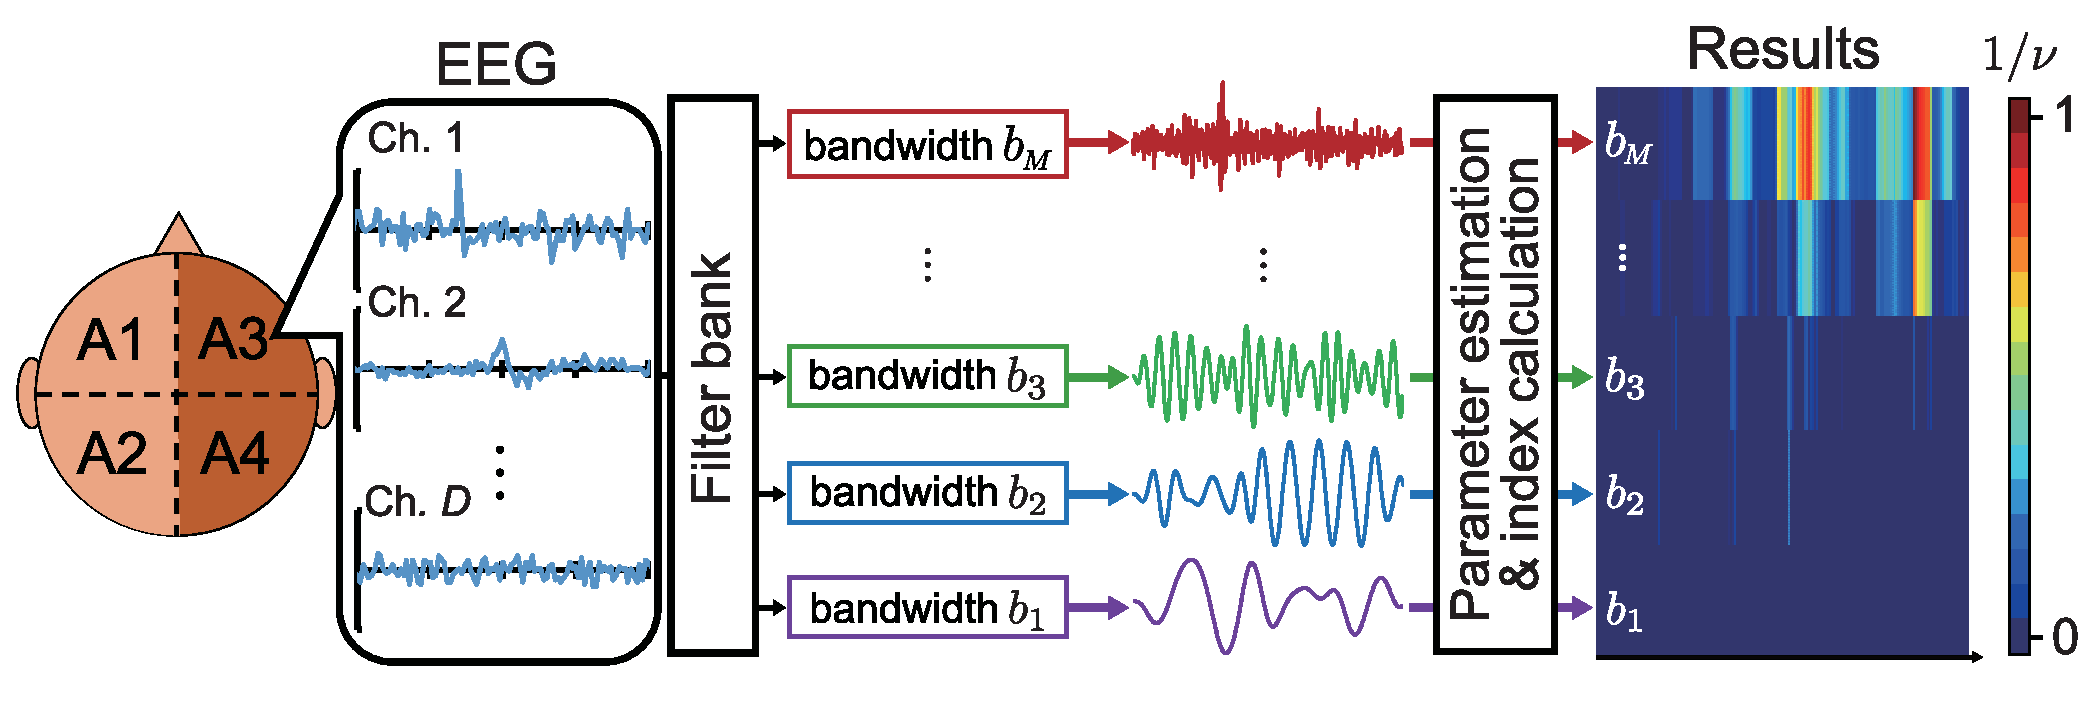
\includegraphics[width=0.8\hsize]{figure/system_5.eps}
%\end{center}
\caption{Overview of the proposed analysis method. The recorded EEG signals are decomposed into multiple frequency bands ($b_1$--$b_M$) by using a filter bank consisting of parallel band-pass filters. 
The evaluation index $1/\nu$ is then calculated for each frequency band, based on the parameter estimation results of the proposed model.
The results are shown as a color map.}
\label{fig:system}
\end{figure*}
%%%%%%%%%%%%%%%%%%%%%%%%%%%%%%%%
Fig.~\ref{fig:system} shows an overall outline of the proposed analysis method.
In the proposed method, observed EEG signals are decomposed into multiple frequency bands by using a filter bank consisting of parallel band-pass filters.
Additionally, we estimate non-Gaussianity for signals in each frequency band based on the proposed multivariate scale mixture model.

First, the EEG signal at time $t$ recorded from the $D$ pair of electrodes is defined as $\mathbf{x}_t \in \mathbb{R}^D$. 
Then, $\mathbf{x}_t$ is divided into $M$ frequency bands ($b_1, \cdots, b_M$) by applying a filter bank consisting of a third-order Butterworth band-pass filter to the signal; the obtained signal is defined as $x_t^{(b_m)}$ ($m = 1,\cdots, M$).
Second, parameter estimation for the variance-covariance matrix distribution based on the proposed model is performed on $\mathbf{x}^{(b_m)}_t$ for each frequency band, and an $\nu$ characterizing the stochastic fluctuation is obtained.
Because the characteristics of EEG signals change significantly in a time series, a sliding window of length $W$ (s) is applied to $\mathbf{x}^{(b_m)}_t$ in each band, and $\nu$ is estimated from the sample in the window following the procedure described in Section II-\textit{B}.
The time window is slid by $S$ (s) continuously, resulting in the estimation of $ \nu$ in a time series.
%Here, $\nu$ is a parameter that means that the closer to $\infty$, the closer the distribution approaches a Gaussian distribution, that is, the smaller the stochastic fluctuation.

Here, $\nu$ is a parameter that controls the Gaussianity of EEG signals.
The EEG distribution becomes closer to a Gaussian form as the value of $\nu$ approaches $\infty$; that is, the stochastic fluctuation decreases as $\nu$ increases.
In this paper, we calculate $1/\nu$, which is the reciprocal of $\nu$, to provide intuitive meaning and to serve as an index that characterizes the non-Gaussianity. 
The index $1/\nu$ indicates that the larger its value, the larger the stochastic fluctuation of the EEG signal.

From the above, it is clear that the stochastic fluctuations latent in each frequency band of EEG signals can be estimated continuously.
It is also possible to obtain the spatial distribution of stochastic fluctuations by dividing the EEG electrode arrangement into multiple regions in advance and performing the above analysis for each region.


\section{Experiments}
%%%%%%%%%%%%%%%%%%%%%%%%%%%%%%%%
\begin{figure}[!t]
\centering
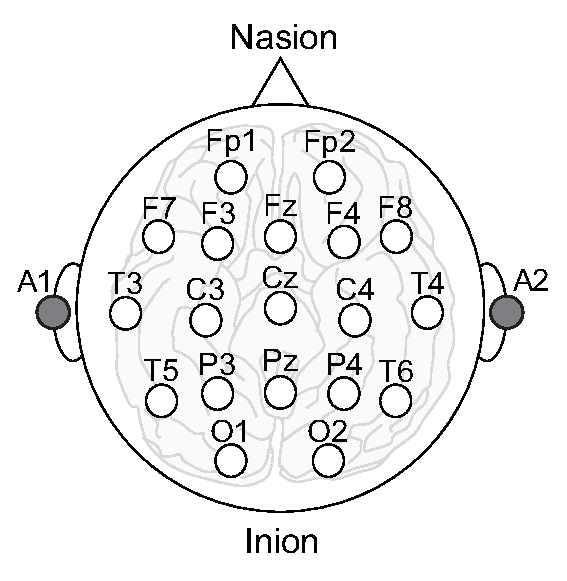
\includegraphics[width=0.5\hsize]{figure/electrodes.eps}
%\end{center}
\caption{International 10--20 electrode montage}
\label{fig:electrodes}
\end{figure}

\subsection{Simulation}
To verify the accuracy of parameter estimation based on the proposed model, we performed a simulation experiment to evaluate the error rate between the true and estimated values of the parameters.
Using the fact that the marginal distribution of the proposed model is equivalent to the multivariate Student-$t$ distribution, a random number sequence $\{\mathbf{x}_t \in \mathbb{R}^D; t = 1, \cdots, T\}$ following a Student-$t$ distribution $\mathrm{St}(\mathbf{x}_t|\nu'_0, \mathbf{\Psi}'_0)$ was generated.
Here, the $\{\mathbf{x}_t \}$ values were regarded as a time series of an EEG signal recorded at a sampling frequency of $f_s$.
The accuracy of the distribution estimation was verified by comparing true values $\nu_0$ and $\mathbf{\Psi}_0$ with estimated values $\nu$ and $\mathbf{\Psi}$, after converting $\nu'_0$ and $\mathbf{\Psi}'_0$ to inverse Wishart distribution parameters based on (\ref{eq:eq6}) and (\ref{eq:eq7}).
As an index of estimation accuracy for each parameter, the absolute percentage error was defined as ${|\nu_0 -\nu|}/{|\nu_0|}\times100$ and ${\|\mathbf{\Psi}_0-\mathbf{\Psi}\|_F}/{\|\mathbf{\Psi}_0\|_F}\times100$.
$\|\mathbf{\Psi}\|_F$ is the Frobenius norm~\cite{GeneHowardGolub2013} of $\mathbf{\Psi}$ and is obtained as
%
\begin{align}%ディスプレイ用番号付き12
	\|\mathbf{\Psi}\|_F=\sqrt{\sum_{i=1}^D \sum_{j=1}^D |{\psi_{ij}}|^2},
\end{align}
%
where ${\psi_{ij}}$ is the element of $\mathbf{\Psi}$.
In the estimation of each parameter, the first $W$ values of the signals $\{\mathbf{x}_t \}$ were used.
The window length $W$ took values of 1, 2, 5, 10, 15, 20, 30, 50, and 100 s, and the number of dimensions $D$ took values of 1, 2, 4, 8, 16, and 19.
The average absolute percentage errors were calculated by changing the true values of multivariate $t$-distribution parameters 400 times ($\nu'_0 = 0.5, 1.0, 1.5, \cdots, 10.0, {\psi'_0}_{ii} = 1.0, 2.0, 3.0, \cdots, 20.0$).
Note that $\mathbf{\Psi}'_0$ was changed only in terms of its diagonal components ${\psi'_0}_{ii}$, and the off-diagonal components were fixed at 0.5.
The $T$ and $f_s$ values in artificial data generation were set as 100 s and 500 Hz.

\subsection{EEG analysis}
To evaluate the validity of the proposed model and the effectiveness of the proposed index $1/\nu$ for epileptic seizure detection, analysis experiments were conducted.
Twenty epileptic patients with focal epilepsy participated in the experiments.
Table~\ref{table:conditions} contains patient information, analysis times, and the durations of the epileptic seizures.
The EEG signals were recorded with a digital sampling frequency of 500 Hz using an electroencephalograph system (Neurofax EEG-1218, Nihon Kohden, Tokyo, Japan) while the patients were in the supine position.
The 19-channel surface electrodes ($D=19$) were placed on the scalp according to the international 10--20 electrode system, with reference electrodes on both earlobes: A1 and A2 (see Fig. \ref{fig:electrodes}).
The experiments were approved by the Okayama University Ethics Committee (approval No: 1706-019). The onset and offset of a focal seizure in each EEG recording were marked by a board-certified epileptologist (T.A.).
% (承認番号:研1706-019).
%%%%%%%%%%%%%%%%%%%%%%%%%%%%%%%%

%=====================
%Table1 被験者
%=====================
\begin{table}[!t]
\centering
 \caption{Patient conditions}
 \label{table:conditions}
% \vspace{-2.5mm}
% \scalebox{1.1}[1.1]{%size
  \begin{tabular}{lllll}%{ccccc}
   \toprule %booktabs
   \multirow{2}{*}{Patient} &  \multirow{2}{*}{Sex} &  Age  & Total data & Seizure \\
   & & (year) &  length (s) & duration (s) \\
   \midrule %booktabs
   A & Male & 2 & 300 & 71\\ %AS
   B & Male & 23 & 300 & 54\\ %ZX
   C & Male & 2 & 300 & 31\\ %AR
   D & Male & 4 & 380 & 93\\ %IP
   E & Female & 31 & 320  & 39\\ %IQ
   F & Male & 41 & 300 & 32\\%M0 20190918
   G & Female & 3 & 240 & 53\\%62 20191209
   %Sub. F & Male & 0.5 & 500 & 158\\ %IS省くかも20190716 20190918省く!!
   %Sub. G & Female & 14 & 420 & 72\\ %IT省くかも2019071	6 20190918省く!!
   H & Male & 19 & 390 & 36\\ %IV
   I & Male & 0.8 & 360  & 98\\ %15
   J & Male & 20 & 390 & 16\\ %IW
   K & Male & 36 & 300 & 23\\ %NR
   L & Male & 9 & 300 & 43\\ %NS
   M & Male & 13 & 300  & 43\\ %ZR
   N & Male & 15 & 300 & 48\\%61 20191209
   %Sub. N & Male & 12 & 300 & 88\\ %ZS
   O & Male & 8 & 300 & 17\\ %ZT
   P & Female & 19 & 300 & 69\\ %ZV
   Q & Male & 27 & 420 & 62\\ %AB
	 R & Male & 38 & 300 & 65\\ %ZY
	 S & Male & 17 & 300 & 17\\ %ZZ
	 T & Male & 19 & 300 & 65\\ %00
   \bottomrule %booktabs
  \end{tabular}
%  }
\end{table}

%=====================

First, the proposed model was fitted to the recorded EEG signals for all participants, and the index $1/\nu$ was calculated.
We set the frequency bands in the proposed method to $b_m \in\{\delta, \theta, \alpha,\beta, \gamma\}$, and decomposed EEG signals into $\delta$ (1--3 Hz), $\theta$ (4--7 Hz), $\alpha$ (8--12 Hz), $\beta$ (13--24 Hz), and $\gamma$ (25--100 Hz).
These frequency bands are generally used to extract features of EEG signals~\cite{ep1994}.
Here, the fitting of the model and the calculation of $1/\nu$ were performed continuously using a sliding window with a length of $W$ = 15 s and a sliding width of $S$ = 1 s.

We then performed a goodness-of-fit test to validate the proposed model for EEG signals in each frequency band.
As an evaluation index for the goodness-of-fit, we used the Bayesian information criterion (BIC)~\cite{Schwarz1978}, which balances the fitness and complexity of the model.
%
\begin{align}%ディスプレイ用番号付き12
	\mathrm{BIC} = -2 \mathrm{ln}L(\hat{\theta}) + k \mathrm{ln}(N_W).
\end{align}
%
Here, $\mathrm{ln}L(\hat{\theta})$ is the log-likelihood of the model, $k$ is the number of estimated parameters in the model, and $N_W$ is the sample size in the sliding window. 
BIC was calculated for the fitting results for each sliding window.
For comparison, BIC was also calculated for a multivariate Gaussian distribution model and a multivariate Cauchy distribution model, which has a heavier tail than the Gaussian distribution.

Next, to verify the effectiveness of the evaluation of EEG non-Gaussianity based on the proposed method, we investigated whether epileptic seizures and non-seizures were classified accurately by using the calculated indices $1/\nu$ of each frequency band ($\delta$--$\gamma$ bands). 
The calculated $1/\nu$ results for each patient were divided into those obtained from seizure segments and those obtained from non-seizure segments.
Here, a non-seizure segment is defined as the period from the start of the recording to the onset of seizures.
Non-seizure segments that included extraneous noise owing to unexpected body movements or electrode shifts in the original EEG signals were excluded from the analysis.
In addition, beacause the sample size for calculating $1/\nu$ differed significantly between the seizure and non-seizure segments, the calculated $1/\nu$ in the non-seizure segment was randomly sampled based on the sample size for calculating $1/\nu$ in the seizure segment, and the sample size for calculating $1/\nu$ in both sections was made uniform for each patient.

As an evaluation index of classification performance, we calculated the area under the curve (AUC) based on a receiver operating characteristic (ROC) analysis.
The AUC is an evaluation scale calculated from the ROC curve plotting the relationship between the false positive rate and the true positive rate.
The closer the AUC value is to 1, the higher the classification performance.
For comparison, the AUC was calculated in the same manner using only the EEG amplitude information.
The root mean square (RMS)~\cite{Hamedi2014} was used for the amplitude information:
%
\begin{equation}%ディスプレイ用番号付き12
		\mathrm{RMS} = \sqrt{\frac{1}{N_W} \sum_{i=1}^{N_W} (x_i^\mathrm{Cz})^2},
\end{equation}
%
where $x_i^\mathrm{Cz}$ is an EEG signal at the Cz channel (see Fig.~\ref{fig:electrodes}) obtained from the top of the head.
This RMS was calculated continuously using a sliding window with the same settings as those used in calculating $1/\nu$.

%%%%%%%%%%%%%%%%%%%%%%%%%%%%%%%%
\begin{figure}[t]
\centering
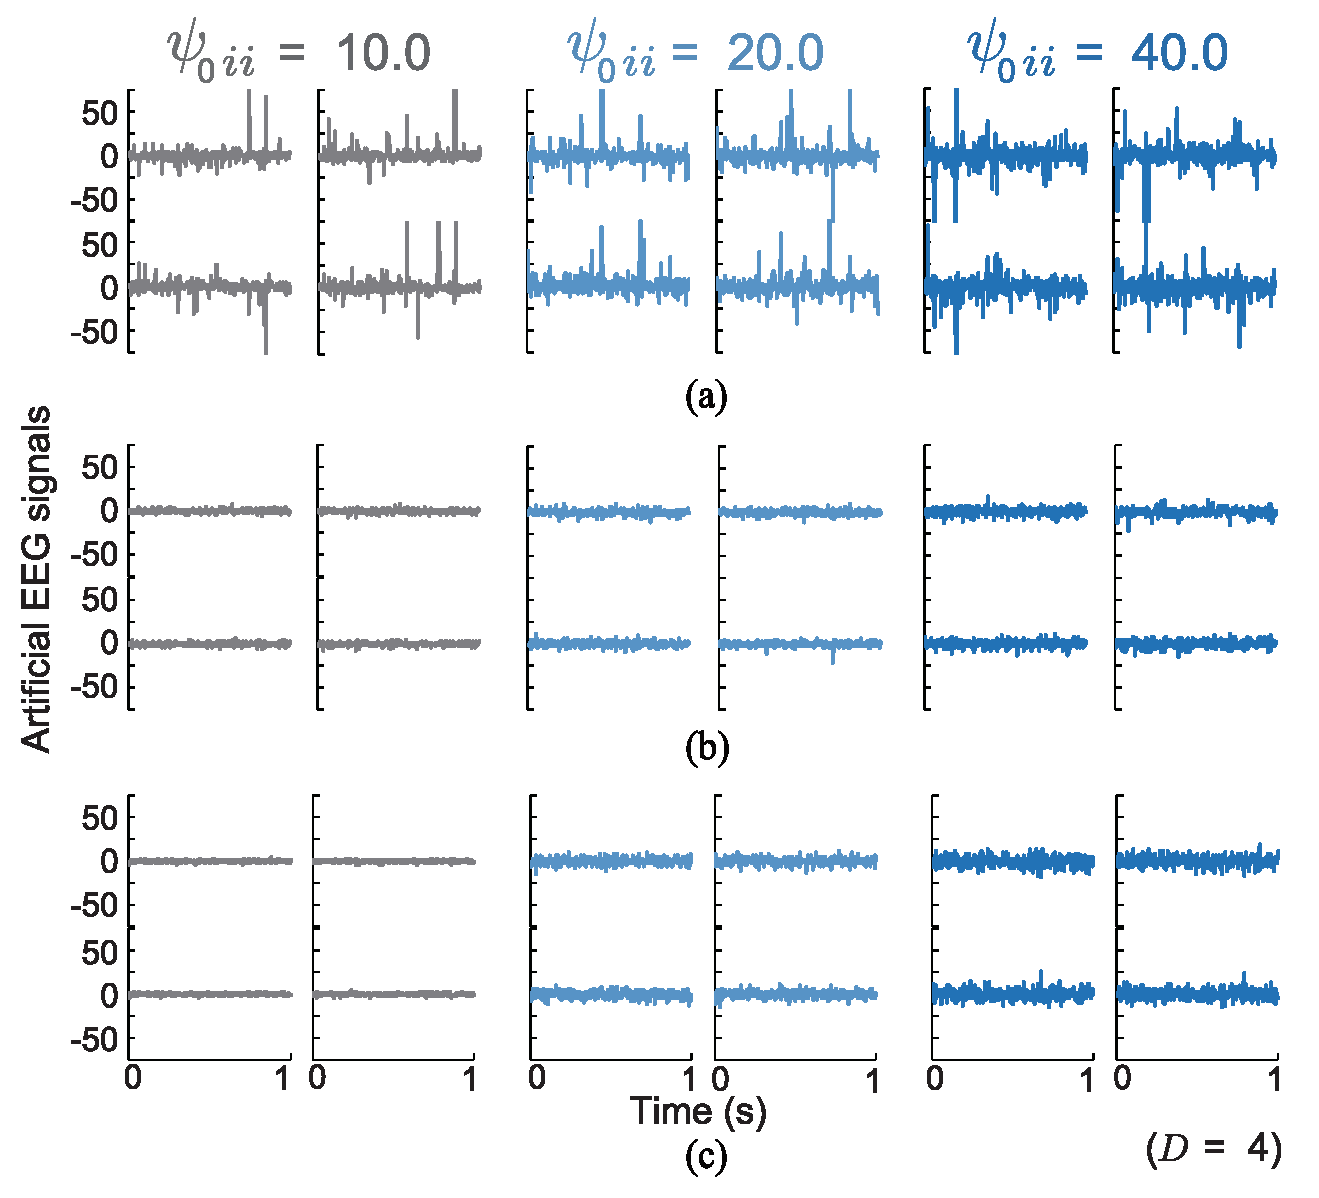
\includegraphics[width=1.0\hsize]{figure/simulation_EEG_4.eps}
%\end{center}
\caption{Examples of artificially generated EEG signals ($D$ = 4) with $\nu_0$ set to (a) $\nu_0 = 5.0$, (b) $\nu_0 = 8.0$, and (c) $\nu_0 = 13.0$; in each case, ${{\psi_0}_{ii}}$ was set to ${{\psi_0}_{ii}} = 10.0$, ${{\psi_0}_{ii}} = 20.0$, and ${{\psi_0}_{ii}} = 40.0$.}
\label{fig:sim_EEG}
\end{figure}
%%%%%%%%%%%%%%%%%%%%%%%%%%%%%%%%

%%%%%%%%%%%%%%%%%%%%%%%%%%%%%%%%
\begin{figure}[!t]
\centering
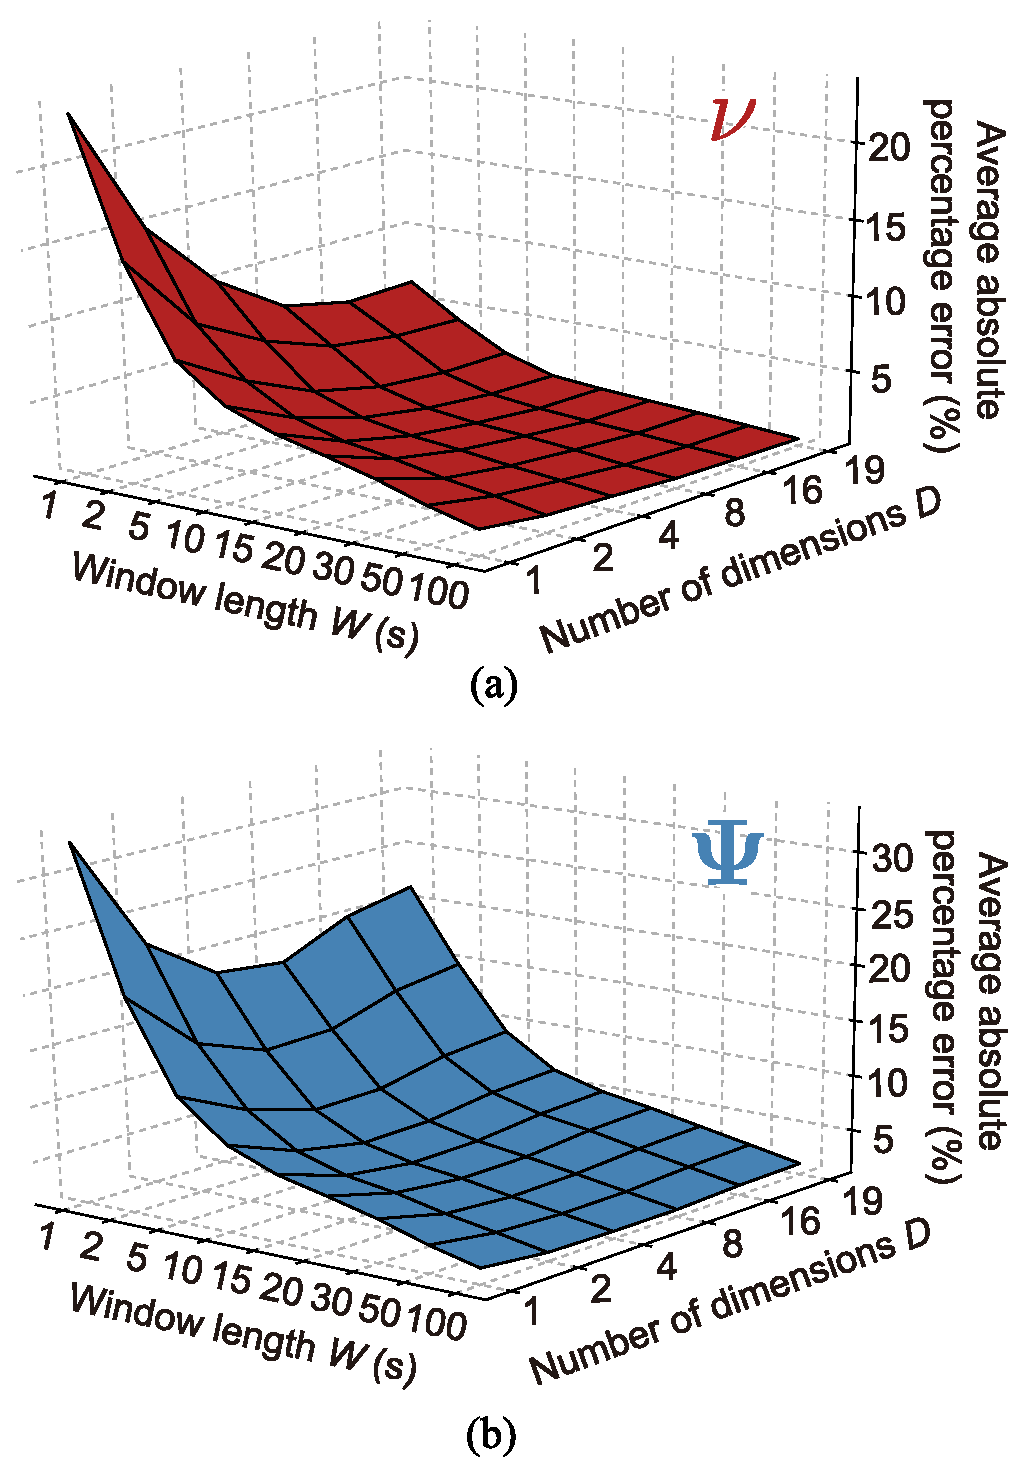
\includegraphics[width=0.8\hsize]{figure/AAPE_color_dim_fro_time_ver3.eps}
%\end{center}
\caption{Average absolute percentage errors for each combination of the number of input dimensions ($D$) and the sliding window length ($W$) in the estimation of variance-covariance distribution parameters. (a) Degrees of freedom $\nu$. (b) Scale matrix $\mathbf{\Psi}$.}
\label{fig:ES_param}
\end{figure}
%%%%%%%%%%%%%%%%%%%%%%%%%%%%%%%%

\section{Results}
%\subsection{Simulation}

In the simulation experiments, we generated time-series simulation data and verified the estimation accuracy of the distribution parameter.
Fig. \ref{fig:sim_EEG} shows examples of time-series waveforms of $\mathbf{x}_t$, where the parameters of the inverse Wishart distribution used in artificial data generation were set as $\nu_0$ = 5.0, $\nu_0$ = 8.0, and $\nu_0$ = 13.0, and ${\psi_0}$ was changed to ${\psi_0}_{ii}$ = 10.0, ${\psi_0}_{ii}$ = 20.0, and ${\psi_0}_{ii}$ = 40.0 for each $\nu_0$.
In the examples, the number of dimensions for artificial EEG signals is set to $D = 4$, and the signals for each dimension are shown.
The vertical and horizontal axes indicate the signal values and time, respectively. 
Fig. \ref{fig:ES_param} shows the average absolute percentage errors in the estimation of $\nu$ and $\mathbf{\Psi}$ resulting from changing the window length $W$ and the number of dimensions $D$.


%%%%%%%%%%%%%%%%%%%%%%%%%%%%%%%%
\begin{figure*}[!ht] %17名
\centering
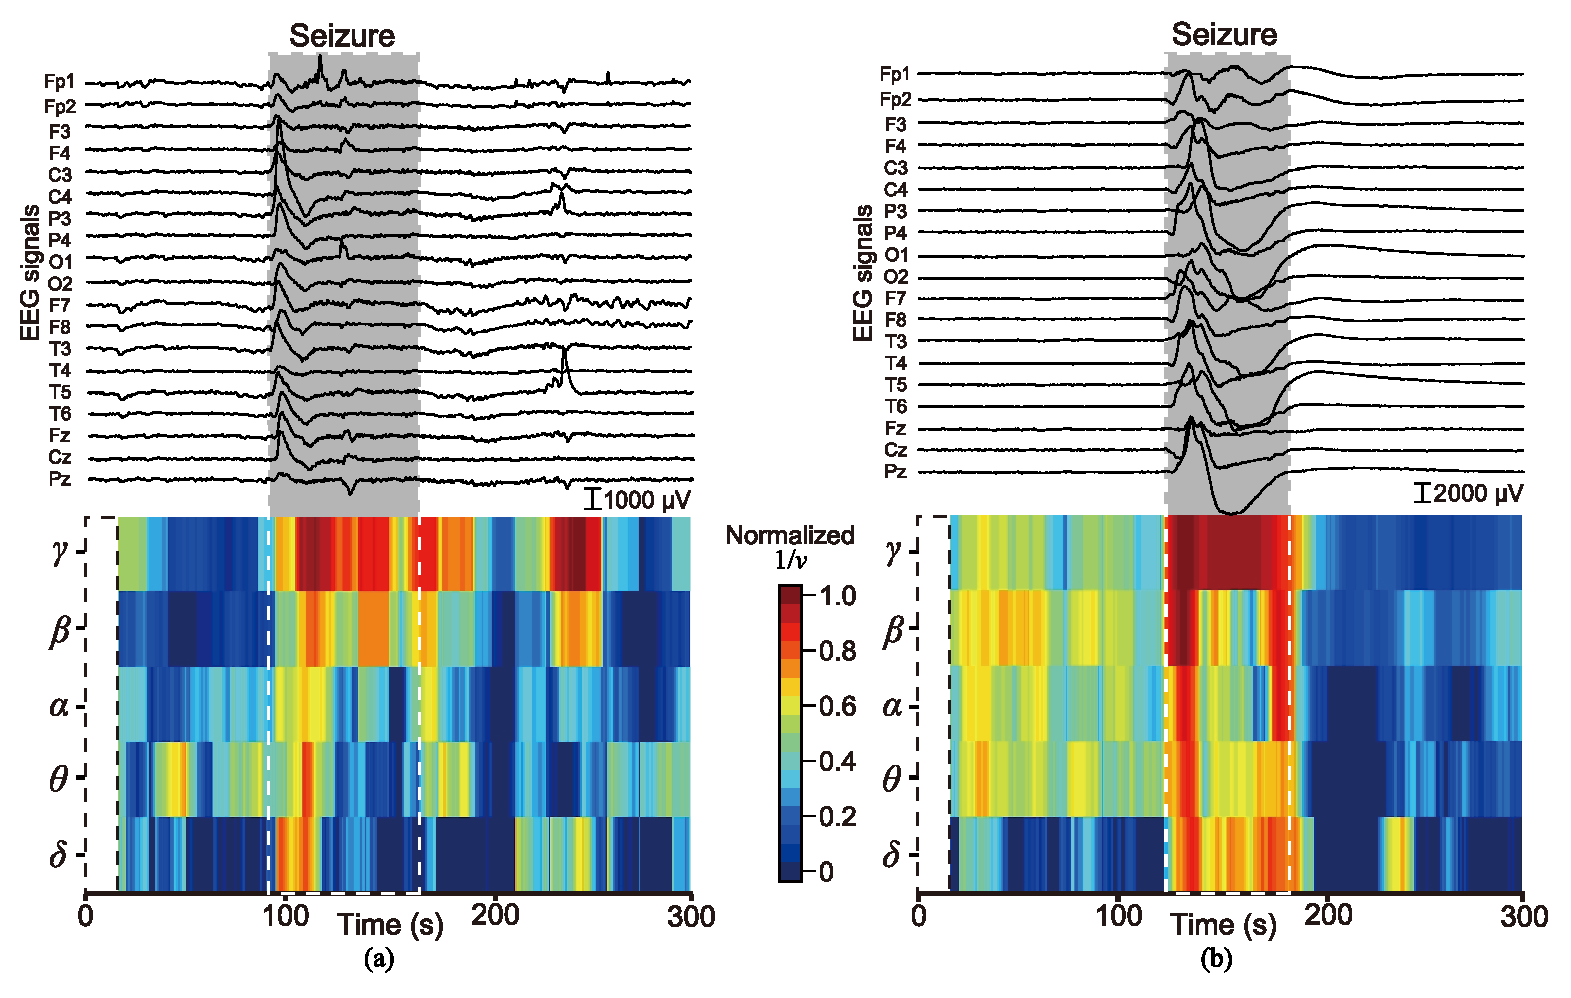
\includegraphics[width=0.9\hsize]{figure/Colormap_ver4_5.eps}
%\end{center}
\caption{Raw EEG signals and corresponding analysis results from the proposed method for (a) patient A and (b) patient B.
Proposed index $1/\nu$ was normalized based on min-max normalization, rescaling the range of features to scale the range in [0, 1].  }
\label{fig:Colormap}
\end{figure*}
%%%%%%%%%%%%%%%%%%%%%%%%%%%%%%%%

%\subsection{EEG analysis}
In the EEG analysis experiments, we performed a goodness-of-fit test for EEG signals and evaluated non-Gaussianity using the proposed index.
Table \ref{table:BIC} shows the percentage of times that the BIC of each model became a minimum in the EEG signals of the $\delta$--$\gamma$ bands.
The table also shows the results of the McNemar test (significance level: 1\%) adjusted by the Holm method using the proposed model as a control group.
In all frequency bands, significant differences were observed between the proposed model and the other models ($p < 0.001$).
In Fig. \ref{fig:Colormap}, color maps show the $1/\nu$ calculations corresponding to the raw EEG waveforms of patient A and patient B.
In the color maps, $1/\nu$ was normalized to ensure that the maximum value of all frequency bands would be 1 and the minimum value would be 0.
The shaded areas in the waveforms and the areas surrounded by white dotted lines indicate epileptic seizure occurrences diagnosed by an epileptologist.

Fig. \ref{fig:dens} shows the $1/\nu$ distribution in each frequency band for all patients, as calculated by kernel density estimation~\cite{Parzen1962} for each seizure and non-seizure segment.
The figure also shows the results of the paired $t$-test (significance level: 1\%) and the effect size $g$~\cite{Hedges1981} between the $1/\nu$ distributions from seizure and non-seizure segments.
Here, the effect size $g$ is a statistical index indicating the magnitude of the difference between the mean values of the two distributions.
In general, $0.2 \leq g < 0.5$ is interpreted as a small effect size, $0.5 \leq g < 0.8$ is a medium effect size, and $0.8 \leq g$ is a large effect size~\cite{Cohen2013}.

%%%%%%%%%%%%%%%%%%%%%%%%%%%%%%%%
\begin{figure}[!t] %20名
\centering
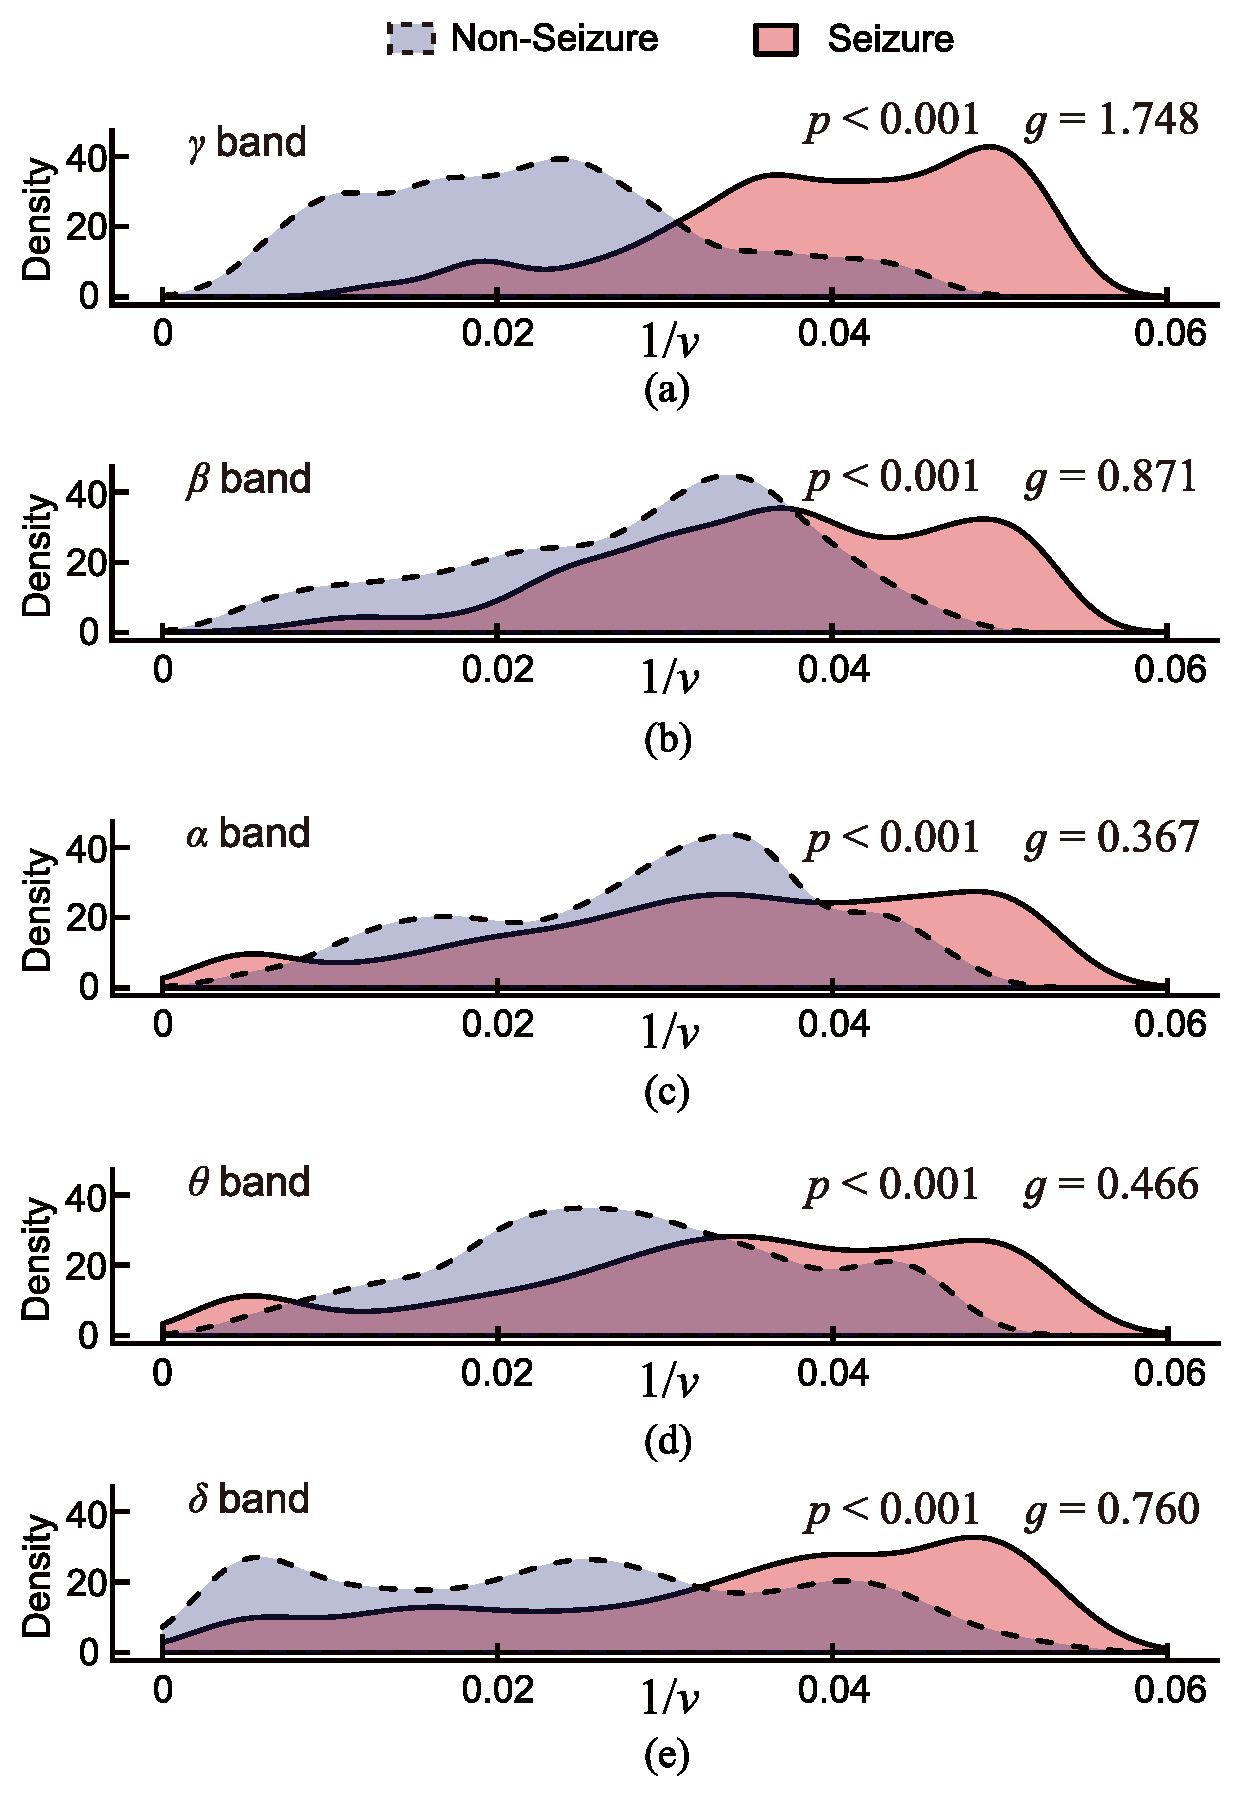
\includegraphics[width=1.0\hsize]{figure/dens_test_20_ver4.eps}
%\end{center}
\caption{Experimental $1/\nu$ distributions estimated from EEG signals. The \textit{p}-value from the paired $t$-test and the effect size \textit{g} are also shown. (a) $\gamma$ band. (b) $\beta$ band. (c) $\alpha$ band. (d) $\theta$ band. (e) $\delta$ band.}
\label{fig:dens}
\end{figure}
%%%%%%%%%%%%%%%%%%%%%%%%%%%%%%%%

Fig. \ref{fig:roc}(a) shows the ROC curves obtained via seizure and non-seizure classification based on the $1/\nu$ in each frequency band and by using RMS as amplitude information.
The AUCs obtained from the ROC curves are shown in Fig. \ref{fig:roc}(b).
The AUCs of $1/\nu$ in each frequency band ($\delta$--$\gamma$) were 0.709, 0.647, 0.615, 0.727, and 0.881, respectively, and the AUC of RMS was 0.816.
A Delong's test~\cite{Delong1988} with the Holm adjustment (significance level: 1\%) was performed to test the AUCs between the $1/\nu$ in each band and the RMS used as the conventional feature representing the amplitude (i.e., the AUC of RMS was set as a control group).
There were significant differences between the AUCs of $1/\nu$ in each band and the AUC of RMS ($p < 0.001$).


%%%%%%%%%%%%%%%%%%%%%%%%%%%%%%%%
\begin{figure}[!t] %20名
\centering
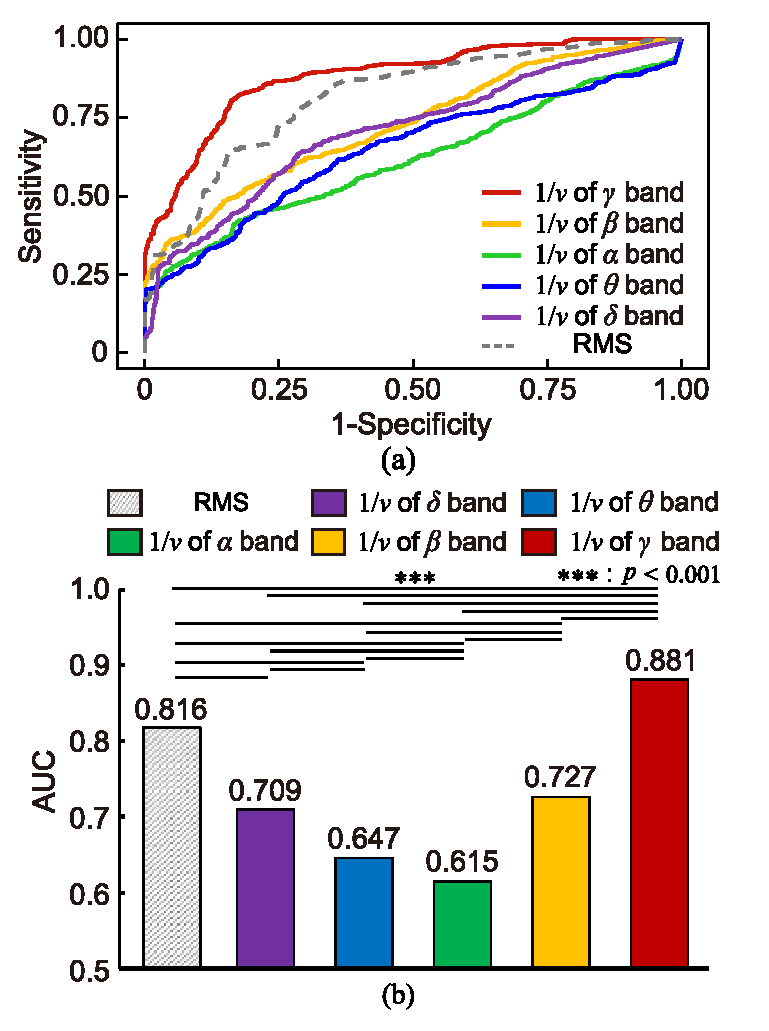
\includegraphics[width=0.85\hsize]{figure/ROC_rms_ver10.eps}
%\end{center}
\caption{Results of ROC analysis based on $1/\nu$ for each frequency band and RMS.
(a) ROC curves for seizure and non-seizure segments.
(b) Calculated AUC for seizure and non-seizure segments.
The pairwise comparisons between RMS and the other results based on the Delong's test for two correlated ROC curves with the Holm adjustment are also shown ($p<0.001$).}
\label{fig:roc}
\end{figure}
%%%%%%%%%%%%%%%%%%%%%%%%%%%%%%%%

\section{Discussion}
In the simulation experiment, as the value of $\nu_0$ changes from $\nu_0 = 5.0$ to $\nu_0 = 13.0$, it can be seen that the outlier-like variance of the waveform does not appear frequently, and the waveform stabilized (Fig.~\ref{fig:sim_EEG}). 
This indicates that the distribution approaches a Gaussian distribution as $\nu$ increases, because this parameter determines the Gaussianity of the distribution.
It can also be seen that the amplitude of the artificial data increases as the value of ${\psi_0}_{ii}$ changes from ${\psi_0}_{ii}=10.0$ to ${\psi_0}_{ii}=40.0$.
This is because $\psi_{ii}$, the diagonal component of $\mathbf{\Psi}$, is a parameter that characterizes the scale of the variance of EEG signals in each dimension.

The average absolute percentage errors in the estimation of $\nu$ and $\mathbf{\Psi}$ are approximately 2\% at $W$ = 100 s, which indicates that the estimation is accurate (Fig.~\ref{fig:ES_param}).
However, the error rate increases as the window length $W$ decreases; the error rate is approximately 25\% in $\nu$ and approximately 35\% in $\mathbf{\Psi}$ at $W$ = 1 s.
These results indicate that the estimation accuracy depends on the window length used for parameter estimation. 
When the number of dimensions was increased, the average absolute percentage error of $\nu$ decreased, and that of $\mathbf{\Psi}$ decreased initially and then increased again. 
Here, $\nu$ is a one-dimensional parameter defined for all input dimensions; therefore, it is considered that increasing the number of dimensions substantially increased the sample size used in the estimation of $\nu$, thereby decreasing the average absolute percentage error in the estimation. 
The scale matrix $\mathbf{\Psi}$ is affected by the estimation result of $\nu'$ because $\mathbf{\Psi} = \nu' \mathbf{\Psi}'$; therefore, the estimation error of $\mathbf{\Psi}$ is considered to decrease synergistically when the number of dimensions increases. 
Indeed, the estimation error decreased as the number of dimensions ranged from $D = 1$ to $D = 8$, whereas it increased as the number of dimensions ranged from $D = 8$ to $D = 16$.
This is probably because the calculation of the average absolute percentage error was performed using the Frobenius norm. Even if the estimation accuracy for each element in the matrix does not change, the overall error increases as the number of elements increases with increases in the number of dimensions.
%=====================
%Table1 BIC
%=====================
\begin{table}[!t]
\centering
 \caption{Percentage of times each model was selected for different frequency bands based on BIC.}
  \label{table:BIC}
 \begin{threeparttable}
  \begin{tabular}{llll}%{cccc}
   \toprule %booktabs
    & &\;{Model}&\\ \cmidrule(r){2-4}
   {Frequency band} & {Proposed} & \; Gaussian & Cauchy \\
   \midrule %booktabs
   $\delta$ (1--3 Hz) & 81.80\%  &\; 17.92\% *** &0.28\% ***\\ %6110
   $\theta$ (4--7 Hz) & 95.47\%  &\; 4.42\% *** &0.11\% ***\\ %6110
   $\alpha$ (8--12 Hz) & 96.79\%  &\; 3.09\% *** &0.12\% ***\\ %6110
   $\beta$ (13--24 Hz)  & 99.05\%  &\; 0.59\% *** &0.36\% ***\\ %6110
   $\gamma$ (25--100 Hz) & 99.28\%  &\; 0.21\% *** &0.51\% ***\\ %6110
   %1 & 58.24 \%  & 41.72 \%  & 0.04 \% & 51.57 \%  & 48.32 \%  & 0.11 \% \\ %5726
   %5 & 97.04 \%  & 2.90 \%  & 0.06 \%  & 95.01 \%  & 4.87 \%  & 0.12 \%  \\ %6074
   %10 & 99.52 \%  & 0.35 \%  & 0.13 \% & 99.06 \%  & 0.57 \%  & 0.37 \% \\ %5979
   %15 & 99.82 \%  & 0.08 \%  & 0.10 \% & 99.48 \%  & 0.21 \%  & 0.31 \% \\ %6170
   \bottomrule %booktabs
   \addlinespace[1.0mm]
  \end{tabular}
    \begin{tablenotes}[para,flushleft]
  ***: significant difference with the proposed model as indicated by a McNemar test with a Holm adjustment (\textit{p} $<$ 0.001)
  \end{tablenotes}
  \end{threeparttable}
\end{table}

%=====================

From the above, it is clear that as the window length increases, the estimation of $\nu$ and $\mathbf{\Psi}$ is performed more accurately.
As the number of input dimensions increases, the estimation of these parameters is also performed more accurately; however, the estimation accuracy of $\mathbf{\Psi}$ decreases for higher-dimensional inputs.
Additionally, assuming the use of an international 10--20 electrode montage (i.e., the input signal has 19 dimensions), the model parameters can be estimated with an error rate of 10\% or less when the window length exceeds 5 s. 
In particular, setting the window length to 15 s can reduce the error rate to 5\%.

The EEG analysis experiment showed that the proposed model is selected the greatest number of times in all frequency bands based on BIC (Table \ref{table:BIC}).
However, the ratio of the minimum BIC of the multivariate Gaussian distribution model was 17.92\% in the $\delta$ band, which was relatively higher than the others.
One possible explanation is that the distribution shape for each window length differs significantly in the low-frequency bands.
%In addition, it is considered that a multivariate Gaussian distribution model has a higher goodness-of-fit because the number of estimated  parameters in the proposed model ($k_t=382$) is one greater than that in a multivariate Gaussian distribution model ($k_t=381$). 
In addition, the number of parameters in the proposed model ($k = 382$) is slightly higher than that  the multivariate Gaussian distribution model ($k = 381$).
Accordingly, when the signal fits both the proposed model and the Gaussian model almost equally, the Gaussian model, a simpler model, shows better goodness-of-fit owing to the nature of BIC.
However, in the other frequency bands, the percentage at which the proposed model was selected based on the minimum BIC exceeds 95\%.
This is because the proposed model can change parameter $\nu$ to adapt to the shape of EEG distributions (i.e., Gaussianity) that change momentarily according to the state of brain activity.
In contrast, the Gaussian model and Cauchy model have only a certain Gaussianity, and these two models are included in the proposed model as special cases (Gaussian: $\nu \rightarrow \infty$, Cauchy: $\nu = D$).
%It is considered that the proposed model can adapt to a multivariate Gaussian distribution model and a multivariate Cauchy distribution model with a heavy tail by changing the parameter $\nu$ of the proposed model. 
From the above, we can conclude that the proposed model is more suitable for EEG signals than the other models.
In addition, the ratio of the minimum BIC of the proposed model increases as the frequency band becomes higher.
This is because the EEG distribution changes depending on frequency characteristics, and those of high-frequency bands (at which signals change rapidly) are better fitted to the proposed model.

In Fig.~\ref{fig:Colormap}, the $1/\nu$ in the high-frequency band is particularly large in the epileptic seizure segments.
This can be confirmed from the results of all patients; therefore, the proposed method can quantitatively evaluate the change in non-Gaussianity during epileptic seizures as stochastic fluctuations.
However, at approxiamtely 220 s in Fig. \ref{fig:Colormap}(a), a partial increase in $1/\nu$ was observed in intervals other than epileptic seizure segments.
This may have occurred because of artifacts in high-frequency bands, e.g., electromyograms caused by body movements.
The proposed index, which characterizes stochastic fluctuations, may increase to some extent owing to non-stationary noise components superimposed onto the EEG.
%Thus, it is necessary to examine the analysis results in more detail based on the knowledge of doctors.

In Fig. \ref{fig:dens}, the $1/\nu$ distributions of all patients in each frequency band show that the $1/\nu$ of non-epileptic seizure segments is distributed in a region smaller than 0.05 regardless of the frequency band.
In contrast, the $1/\nu$ of epileptic seizure segments is distributed more widely than that of non-epileptic seizure segments, and this tendency is most noticeable in the high-frequency $\gamma$ band.
This can also be confirmed from the effect size $g$, which is the standardized mean difference between two groups.
It is considered that the $1/\nu$ in the high-frequency band best reflects the characteristics of epileptic seizures because a large effect size was obtained in the $\gamma$ band.
This indicates that EEG signals in the high-frequency band exhibited a strong non-Gaussianity owing to epileptic seizures.
Previous studies reported that the activity in the $\gamma$ band, which is the high-frequency band of EEG signals, becomes intense during epileptic seizures~\cite{Kobayashi2004,Kobayashi2009,Benedek2016}.
The detailed mechanism of such $\gamma$ activity is still unknown; however, activities of inhibitory interneurons and electrical coupling through gap junctions were previously suggested~\cite{Park2012}.
These activities cause intermittent amplitude changes specific to epileptic seizures; consequently, the non-Gaussianity in the high-frequency band may be emphasized and $1/\nu$ increases.

In Fig. \ref{fig:roc}(b), a medium to high AUC of 0.881 was obtained in the high-frequency $\gamma$ band, showing that $1/\nu$ in the $\gamma$ band had the highest classification performance. 
In addition, significant differences were noted with the amplitude feature (i.e., RMS); therefore, the $1/\nu$ in the $\gamma$ band provided better classification ability than the conventional feature. 
It is considered that the scale matrix $\mathbf{\Psi}$, which includes amplitude information, and the proposed index $1/\nu$ reflect the different aspects of EEG activity.
Thus, if we could combine the features defined in the proposed model, higher classification performance would be obtained.

\section{Conclusion}
In this paper, we modeled EEG signals using a multivariate scale mixture model.
In the model, a scalp EEG signal recorded at a certain time using multichannel electrodes follows a multivariate Gaussian distribution, and its variance-covariance matrix is handled as a random variable that follows an inverse Wishart distribution. 
The fluctuation of the variance-covariance matrix can be evaluated based on this stochastic relationship.
We also proposed an EEG analysis method by combining the scale mixture model and a filter bank, and introduced an index $1/\nu$ characterizing the non-Gaussianiy.
In this method, EEG signals are decomposed into several frequency bands, and the index for each frequency band was calculated in time series based on the sliding window.

In the simulation experiment, we evaluated the estimation accuracy of each parameter, and showed that the estimation accuracy changes depending on the sample size and the number of dimensions. 
In experiments using EEG signals that included epileptic seizures, it was demonstrated that the proposed model is the most suitable model for EEGs.
In addition, higher accuracy (AUC = 0.881) in classifying seizure and non-seizure segments was obtained by focusing on the proposed index $1/\nu$ in the $\gamma$ band.

However, the proposed index $1/\nu$ may be affected by artifacts such as electromyograms caused by body movement or stiffness owing to seizures.
Therefore, to apply the proposed method more practically, it will be necessary to introduce an algorithm that detects and removes these artifacts.
In addition, we plan to evaluate another parameter of the inverse Wishart distribution, $\mathbf{\Psi}$, and examine its application to EEGs other than EEGs for the diagnosis of epilepsy.

\appendix[Equivalent expression for multivariate scale mixture model]
This appendix shows that the equivalent of the (\ref{eq:eq9}) and (\ref{eq:eq11}).
Equation (\ref{eq:eq11}) can be calculated as
\begin{align}
	p(&\mathbf{x}_n) \notag \\
	&= \int \mathrm{IG}(\tau_n;\nu'/2,\nu'/2) \mathcal{N}(\mathbf{x}_n|\mathbf{0}, \tau_n \mathbf{\Psi}') \mathrm{d}{\tau_n} \nonumber\\
	&= \int \frac{\left(\frac{\nu'}{2}\right)^{\frac{\nu'}{2}}}{\Gamma \left(\frac{\nu'}{2}\right)} (\tau_n)^{-\frac{\nu'}{2}-1} \mathrm{exp} \left[-\frac{1}{\tau_n} \left(\frac{\nu'}{2} \right) \right] \nonumber\\
	&\quad\times\frac{1}{(2\pi)^{\frac{D}{2}}(\tau_n)^{\frac{D}{2}}|\mathbf{\Psi'}|^{\frac{1}{2}}} \mathrm{exp} \left[-\frac{1}{2}\mathbf{x}_n^\mathrm{T} (\tau_n\mathbf{\Psi'})^{-1} \mathbf{x}_n\right] \mathrm{d}{\tau_n} \nonumber\\
	&=\frac{1}{(2\pi)^{\frac{D}{2}}}\frac{\left(\frac{\nu'}{2}\right)^{\frac{\nu'}{2}}}{\Gamma \left(\frac{\nu'}{2}\right)}\frac{1}{|\mathbf{\Psi'}|^{\frac{1}{2}}} \nonumber\\
	&\quad\times \int (\tau_n)^{-\frac{\nu'+D}{2}-1} \mathrm{exp} \left[-\frac{1}{\tau_n} \left(\frac{\nu' + \Delta'}{2}\right) \right] \mathrm{d}{\tau_n} \nonumber \\
%\end{align}
%Multiply (\ref{eq:20}) of the equation by $\frac{\Gamma \left(\frac{\nu'+D}{2}\right)}{\left(\frac{\nu'+\Delta'}{2}\right)^{\frac{\nu'+D}{2}}} \times \frac{\left(\frac{\nu'+\Delta'}{2}\right)^{\frac{\nu'+D}{2}}}{\Gamma \left(\frac{\nu'+D}{2}\right)}$.
%\begin{align}
    &=\frac{1}{(2\pi)^{\frac{D}{2}}}\frac{\left(\frac{\nu'}{2}\right)^{\frac{\nu'}{2}}}{\Gamma \left(\frac{\nu'}{2}\right)}\frac{1}{|\mathbf{\Psi'}|^{\frac{1}{2}}} \frac{\Gamma \left(\frac{\nu'+D}{2}\right)}{\left(\frac{\nu'+\Delta'}{2}\right)^{\frac{\nu'+D}{2}}}\nonumber\\
	&\quad\times \int \frac{\left(\frac{\nu'+\Delta'}{2}\right)^{\frac{\nu'+D}{2}}}{\Gamma \left(\frac{\nu'+D}{2}\right)} (\tau_n)^{-\frac{\nu'+D}{2}-1} \nonumber\\
	&\quad\times \mathrm{exp} \left[-\frac{1}{\tau_n} \left(\frac{\nu' + \Delta'}{2}\right) \right] \mathrm{d}{\tau_n} \nonumber\\
	&=\frac{1}{(2\pi)^{\frac{D}{2}}}\frac{\left(\frac{\nu'}{2}\right)^{\frac{\nu'}{2}}}{\Gamma \left(\frac{\nu'}{2}\right)}\frac{1}{|\mathbf{\Psi'}|^{\frac{1}{2}}} \frac{\Gamma \left(\frac{\nu'+D}{2}\right)}{\left(\frac{\nu'+\Delta'}{2}\right)^{\frac{\nu'+D}{2}}}\nonumber\\
	&\quad\times \int \mathrm{IG}(\tau_n;\frac{\nu'+D}{2},\frac{\nu'+\Delta'}{2}) \mathrm{d}{\tau_n}.
	\label{eq:20}
\end{align}
Here, the integral of the probability density function over the entire space is equal to 1.
%\begin{align}
%\label{eq:22}
%\int \mathrm{IG}(\tau_n;\frac{\nu'+D}{2},\frac{\nu'+\Delta'}{2}) \mathrm{d}{\tau_n}=1.
%\end{align}
Hence, (\ref{eq:20}) can be expressed in the same form as (\ref{eq:eq9}).
\begin{align}
	p(\mathbf{x}_n) &= \frac{\Gamma(\frac{\nu'+D}{2})}{\Gamma(\frac{\nu'}{2})} \frac{|{\bm \Psi'}|^{-\frac{1}{2}}}{\left(\pi \nu' \right)^{\frac{D}{2}}} \left(1+\frac{\Delta '}{\nu '} \right)^{-\frac{\nu'+D}{2}}.
\end{align}

tmp

%=====================
%Table3 AUC
%=====================
\begin{table}[!t]
\centering
  \caption{AUC of all features for different frequency bands.}
  \label{table:AUC}
  \begin{threeparttable}
  \begin{tabular}{lllll}%{lcccc}
    \toprule %booktabs
    & \multicolumn{4}{c}{Features}\\ \cmidrule(r){2-5}
    {Frequency band} & {$1/\nu$} &  RMS &\textbar ToC\textbar & ApEn \\
    \midrule %booktabs
    $\delta$ (1--3 Hz) & 0.709  & 0.721 &0.757 &0.560\\ 
    $\theta$ (4--7 Hz) & 0.647  & 0.746 &0.717 &0.557\\ 
    $\alpha$ (8--12 Hz) & 0.615  & 0.817 &0.773 &0.555\\ 
    $\beta$ (13--24 Hz)  & 0.727  & 0.822 &0.786 &0.548\\ 
    $\gamma$ (25--100 Hz) & 0.881  & 0.878 &0.853 &0.552\\ 
    \bottomrule %booktabs
    \addlinespace[1.0mm]
  \end{tabular}
  \end{threeparttable}
\end{table}

% if have a single appendix:
%\appendix[Proof of the Zonklar Equations]
% or
%\appendix  % for no appendix heading
% do not use \section anymore after \appendix, only \section*
% is possibly needed

% use appendices with more than one appendix
% then use \section to start each appendix
% you must declare a \section before using any
% \subsection or using \label (\appendices by itself
% starts a section numbered zero.)
%
tmp:
Feature extraction computation time was also evaluated. The computation time in Debug C++ code with Microsoft Visual Studio with Intel® CoreTM i7–6900K CPU @ 3.2GHz with 64GB RAM was calculated. The computation time was calculated 10 times for the sample length of 7500 for 5 frequency bands in parallel computing by changing the number of cores and the average time and its standard error are  shown in Fig. \ref{fig:c_time}. 

%%%%%%%%%%%%%%%%%%%%%%%%%%%%%%%%
\begin{figure}[!t]
\centering
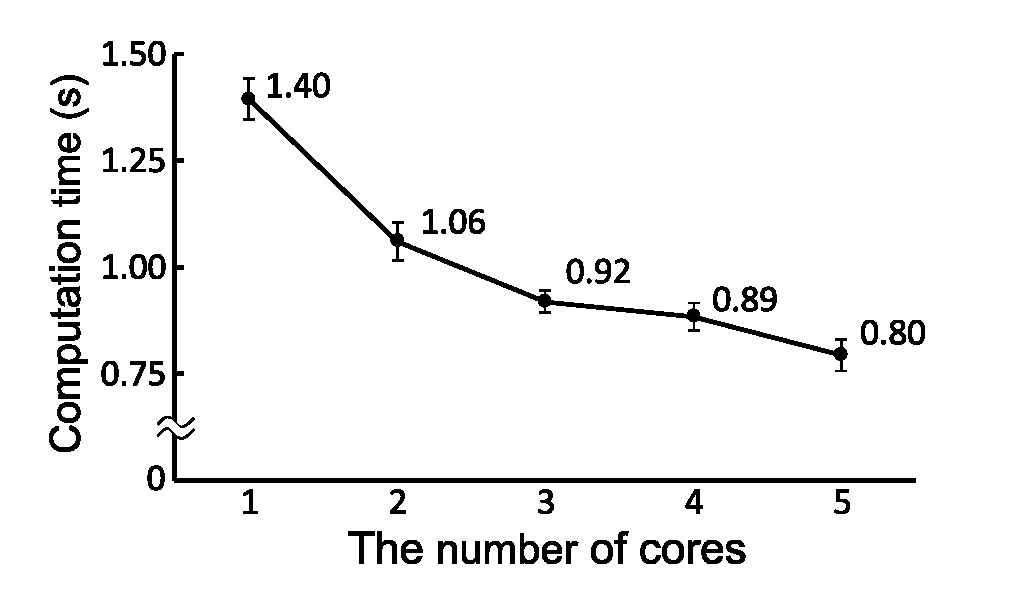
\includegraphics[width=0.9\hsize]{figure/computation_time.eps}
%\end{center}
\caption{The average computation time and its standard error of the proposed index $1/\nu$. The sample length took 7500 ($W$=15), and the nmber of dimensions took $D$=19 by changing the number of cores 1--5.}
\label{fig:c_time}
\end{figure}
%%%%%%%%%%%%%%%%%%%%%%%%%%%%%%%%
% use section* for acknowledgment
%\section*{Acknowledgment}


%The authors would like to thank...


% Can use something like this to put references on a page
% by themselves when using endfloat and the captionsoff option.
\ifCLASSOPTIONcaptionsoff
  \newpage
\fi



% trigger a \newpage just before the given reference
% number - used to balance the columns on the last page
% adjust value as needed - may need to be readjusted if
% the document is modified later
%\IEEEtriggeratref{8}
% The "triggered" command can be changed if desired:
%\IEEEtriggercmd{\enlargethispage{-5in}}

% references section

% can use a bibliography generated by BibTeX as a .bbl file
% BibTeX documentation can be easily obtained at:
% http://mirror.ctan.org/biblio/bibtex/contrib/doc/
% The IEEEtran BibTeX style support page is at:
% http://www.michaelshell.org/tex/ieeetran/bibtex/
%\bibliographystyle{IEEEtran}
% argument is your BibTeX string definitions and bibliography database(s)
%\bibliography{IEEEabrv,../bib/paper}
%
% <OR> manually copy in the resultant .bbl file
% set second argument of \begin to the number of references
% (used to reserve space for the reference number labels box)

\bibliographystyle{IEEEtran}
\bibliography{ref.bib}




% if have a single appendix:
%\appendix[Proof of the Zonklar Equations]
% or
%\appendix  % for no appendix heading
% do not use \section anymore after \appendix, only \section*
% is possibly needed

% use appendices with more than one appendix
% then use \section to start each appendix
% you must declare a \section before using any
% \subsection or using \label (\appendices by itself
% starts a section numbered zero.)
%




% You can push biographies down or up by placing
% a \vfill before or after them. The appropriate
% use of \vfill depends on what kind of text is
% on the last page and whether or not the columns
% are being equalized.

%\vfill

% Can be used to pull up biographies so that the bottom of the last one
% is flush with the other column.
%\enlargethispage{-5in}



% that's all folks
\end{document}
